\documentclass[11pt]{article}
\usepackage[margin=1in]{geometry}
\usepackage{amsmath,amssymb,mathtools,bm}
\usepackage{hyperref}
\usepackage{xcolor}
\usepackage{graphicx}
\usepackage{booktabs}
\usepackage{enumitem}

\newcommand{\dd}{\mathrm{d}}
\newcommand{\D}{\mathrm{D}}
\newcommand{\half}{\tfrac{1}{2}}
\newcommand{\Tr}{\operatorname{Tr}}
\newcommand{\Kn}{\mathrm{Kn}}
\newcommand{\Ma}{\mathrm{Ma}}
\newcommand{\bx}{\bm{x}}
\newcommand{\bu}{\bm{u}}
\newcommand{\bv}{\bm{v}}
\newcommand{\bmlab}{\bm{m}}
\newcommand{\bq}{\bm{q}}

\title{A variational unification of moderate-Knudsen hydrodynamics with
  the phase-space sheet:\\
  the dfmm framework in 1D and 2D, with action-based AMR and
  variance-gamma stochastic dressing}
\author{T.~Abel\\Kavli Institute for Particle Astrophysics and Cosmology\\
  Stanford University and SLAC National Accelerator Laboratory}
\date{Design document, draft of \today}

\begin{document}
\maketitle

\begin{abstract}
We develop a variational discretization of moderate-Knudsen
hydrodynamics that unifies the dfmm one-dimensional moment scheme with
the phase-space sheet picture of collisionless dynamics. The primary
variable is the $4\times 4$ phase-space Cholesky factor $L$ over a
Lagrangian mass-coordinate mesh in two spatial dimensions; in 1D it
reduces to dfmm's existing eight-field scheme. The deterministic
action has connection-form structure with the strain-group $GL(d)$ as
the structure group: covariant derivatives respect tensor weights, and
the Cholesky sector carries a weighted symplectic form $\omega = \alpha^2
\dd\alpha\wedge\dd\beta$ with $\alpha$-local Hamiltonian
$\mathcal{H}_{\rm Ch} = -\half\alpha^2\gamma^2$, generalized to 2D via
principal-axis rotation as $\omega_{2D} = \sum_a \alpha_a^2 \dd\alpha_a
\wedge \dd\beta_a + \omega_{\rm rot}$. The cold-limit reduction is
exact: the action collapses to the mass-coordinate dust action of
Abel--Hahn--Kaehler, and the Hessian degeneracy at $\gamma\to 0$ is
the variational signature of phase-space rank collapse. Stochastic
dressing is added via a generalized Kramers--Moyal action whose
noise variance is variance-gamma distributed; the shape parameter
$\lambda$ is empirically related to the gamma-distribution shape of
compression burst durations, providing a runtime self-consistency
check between the deterministic and stochastic sectors. Bayesian
remap onto an Eulerian quadtree mesh, computed exactly via the r3d
polynomial-moment kernel with curved-element dimension lifting,
implements the law of total cumulants and converts coarse-graining
entropy production into physical phase-space spreading rather than
numerical dissipation. Adaptive mesh refinement is driven by local
discrete action error, unifying shock detection, shell-crossing
detection, and turbulence-cascade detection in a single criterion.
Passive scalar advection is exact at the discrete level by structural
identification with parcel labels. The framework extends naturally to
two-fluid systems via the dfmm modular cross-coupling operator. We
specify the discrete scheme in detail, present a comprehensive
validation hierarchy spanning 1D regression against dfmm benchmarks
through 2D novelty tests including dust-trapping in vortices and
Zel'dovich pancake collapse, and discuss the methods paper structure.
\end{abstract}

\tableofcontents

\section{Introduction}
\label{sec:intro}

Between strictly hydrodynamic and strictly kinetic descriptions of a
fluid lies an intermediate regime of considerable astrophysical
interest. Post-shock relaxation layers, weakly collisional intracluster
plasmas, the cold streams that feed galactic halos, and the multi-stream
regions of cosmological dark matter structure all share a feature: a
local distribution function that is not Maxwellian but also not
arbitrarily structured. Moment closures handle this regime in
principle, but their failure modes are typically invisible to the
scheme itself. The dfmm framework~\cite{dfmm-paper} addresses this
by instrumenting a one-dimensional moment scheme so that closure
quality is reported as part of the output, with three diagnostics
(heat-flux deviation, Cholesky rank-collapse $\gamma$, standardized
skewness $|s|$) that fire on physically distinct failure modes.

This paper extends dfmm in two directions simultaneously. First, we
develop a \emph{variational} formulation in which the deterministic
moment evolution arises as the Euler--Lagrange equations of an action
with connection-form structure, and the stochastic dressing arises
as a generalized Kramers--Moyal MSRJD action with variance-gamma noise
vertices. Second, we extend to two spatial dimensions via the natural
$4\times 4$ phase-space Cholesky factor over Lagrangian space, with
principal-axis decomposition giving a clean structural reduction.

The variational unification has three structural payoffs that are not
available in the original dfmm formulation. (i) The cold-limit
reduction is exact and analytically clean: the action collapses to
the Abel--Hahn--Kaehler mass-coordinate dust action when velocity
dispersion vanishes, and the diagnostic $\gamma\to 0$ acquires a
sharp variational interpretation as Hessian degeneracy of the
deterministic action. (ii) Bayesian remap with the law of total
cumulants converts coarse-graining entropy production into physical
phase-space spreading rather than numerical dissipation, with
exactness through the r3d polynomial-moment kernel. (iii) Passive
scalar advection becomes exact at the discrete level by structural
identification of tracers with parcel labels, addressing a
long-standing pain point of Eulerian schemes in cosmological and
ISM applications.

The paper is structured as follows. Section~\ref{sec:framework}
establishes the variable hierarchy: the $4\times 4$ phase-space
covariance, its Cholesky factorization, and the strain group as a
structure group on the bundle over Lagrangian space.
Section~\ref{sec:action} develops the deterministic action in
connection form, presents the cold-limit reduction, and identifies
the Hessian-degeneracy interpretation of phase-space rank collapse.
Section~\ref{sec:stochastic} develops the generalized Kramers--Moyal
stochastic dressing, derives the variance-gamma noise distribution
from the gamma-distributed burst-duration empirical structure, and
predicts the residual-kurtosis self-consistency check.
Section~\ref{sec:matrix-lift} works out the 2D matrix lift via
principal-axis decomposition. Section~\ref{sec:remap} establishes
the Bayesian remap with law of total cumulants and the r3d
implementation. Section~\ref{sec:tracer} discusses passive scalar
advection. Section~\ref{sec:discrete} specifies the discrete scheme
in 1D and 2D, including polynomial reconstruction with positivity,
discrete Euler-Lagrange equations, action-based AMR, and the implicit
Newton iteration. Section~\ref{sec:two-fluid} extends to two-fluid
systems. Section~\ref{sec:validation} presents the validation
hierarchy and test problem specifications.
Section~\ref{sec:conclusions} summarizes and discusses extensions.

Throughout, we treat the 1D dfmm scheme as the established reference
that the 2D extension must reduce to in the appropriate limits, and
the test-problem hierarchy reflects this: regression against dfmm
benchmarks in 1D mode is a non-negotiable acceptance criterion before
2D claims are made.

\section{Framework: the $4\times 4$ phase-space Cholesky over Lagrangian
  space}
\label{sec:framework}

\subsection{Mass-coordinate Lagrangian space}

Lagrangian space $\mathcal{L}$ is a $d$-dimensional manifold with mass
coordinates $\bmlab{m}\in\mathcal{L}$ ($d=1,2,3$). The fundamental
spacetime field is the position map
\begin{equation}
  \bx(\bmlab,t):\mathcal{L}\times\mathbb{R}\to\mathbb{R}^d,
\end{equation}
with deformation gradient $J^i_{\,j} = \partial x^i/\partial m^j$ and
volume Jacobian $J = \det(J^i_{\,j}) = 1/\rho$. Mass per parcel is
fixed: $\dd m = \rho_0 \dd\xi$ in initial conditions, and
$\rho(\bx,t) = \rho_0/J$ is derived, never stored.

The Lagrangian frame velocity is $\bu = \dot\bx$ at fixed $\bmlab$. The
Eulerian velocity gradient is the connection 1-form on Lagrangian space:
\begin{equation}
  G^i_{\,j}(\bx,t) = \frac{\partial v^i}{\partial x^j}
  = \frac{\partial u^i}{\partial m^k}(J^{-1})^k_{\,j}.
\end{equation}

\subsection{The $4\times 4$ phase-space covariance}

Over each Lagrangian point we attach a phase-space fiber, characterized
at second-moment order by the $2d\times 2d$ covariance matrix
\begin{equation}
  M = \begin{pmatrix} M_{xx} & M_{xv} \\ M_{xv}^\top & M_{vv}\end{pmatrix},
  \qquad M\succeq 0,
  \label{eq:M}
\end{equation}
with each block $d\times d$. Realizability is $M\succeq 0$. The
Cholesky factorization $M = LL^\top$ with $L$ block-lower-triangular
\begin{equation}
  L = \begin{pmatrix} L_1 & 0 \\ L_2 & L_3 \end{pmatrix},
  \quad
  L_1, L_3\in\mathbb{R}^{d\times d}\text{ lower-tri (positive diagonal)},\
  L_2\in\mathbb{R}^{d\times d},
  \label{eq:L-block}
\end{equation}
makes realizability manifest: $M_{xx} = L_1 L_1^\top$,
$M_{xv} = L_1 L_2^\top$, $M_{vv} = L_2 L_2^\top + L_3 L_3^\top$.

In dfmm's 1D specialization, $L_1 = \alpha$, $L_2 = \beta$, $L_3 = \gamma$,
all scalars; the dynamical fields are $(\alpha,\beta)$ with
$\gamma = \sqrt{M_{vv}-\beta^2}$ derived from the EOS. In 2D, $L$ is
a $4\times 4$ lower-triangular matrix with 10 independent components.

\subsection{The strain group as a structure group}

The phase-space covariance transforms as a tensor under the velocity
strain group $GL(d)_v$. Each velocity index carries one factor of
$G$:
\begin{align}
  \mathcal{D}_t M_{xx} &= \dot{M}_{xx}, \notag\\
  \mathcal{D}_t M_{xv} &= \dot{M}_{xv} - G\,M_{xv}, \notag\\
  \mathcal{D}_t M_{vv} &= \dot{M}_{vv} - G\,M_{vv} - M_{vv} G^\top,
  \label{eq:Liouville-cov}
\end{align}
where $\dot{} = \partial_t$ at fixed $\bmlab$. In tensor language, $M_{xx}$
has weight $(0,0)$ under $GL(d)_v$, $M_{xv}$ has weight $(0,1)$,
$M_{vv}$ has weight $(1,1)$. Liouville evolution under collisionless
free streaming is
\begin{equation}
  \mathcal{D}_t M_{xx} = M_{xv} + M_{xv}^\top,\qquad
  \mathcal{D}_t M_{xv} = M_{vv},\qquad
  \mathcal{D}_t M_{vv} = 0.
  \label{eq:Liouville-clean}
\end{equation}
Right-hand sides are algebraic; all strain coupling is absorbed into
the covariant derivative.

\subsection{Specialization to 1D}

With $d=1$, $G = \partial_x u$, weights become integer charges
$q\in\{0,1,2\}$. Charges of the Cholesky factors: $\alpha = L_1$ has
charge $0$, $\beta = L_2$ has charge 1, $\gamma = L_3$ has charge 1.
The covariant derivative is
\begin{equation}
  \mathcal{D}_t^{(q)}\phi = \dot\phi + q (\partial_x u)\phi.
  \label{eq:Dt-1D}
\end{equation}
The dfmm Cholesky equations~\cite{dfmm-paper} become
\begin{equation}
  \mathcal{D}_t^{(0)}\alpha = \beta,\qquad
  \mathcal{D}_t^{(1)}\beta = \frac{\gamma^2}{\alpha} = \frac{M_{vv}(J,s)-\beta^2}{\alpha},
  \label{eq:dfmm-cov}
\end{equation}
recovering the bare-derivative form
\begin{equation}
  \dot\alpha = \beta,\qquad \dot\beta + (\partial_x u)\beta = \gamma^2/\alpha.
  \label{eq:dfmm-bare}
\end{equation}

\subsection{Liouville invariant}

Under collisionless dynamics, the per-parcel phase-space volume
$\sqrt{\det M} = \det L$ is conserved. In 1D this is
$\alpha\gamma = \det L$. In 2D it's the determinant of the $4\times 4$
Cholesky factor. Mass per parcel is fixed by definition, so the full
phase-space volume invariant per unit reference mass is exactly
$\det L$. This is the Liouville invariant we use to characterize the
deterministic dynamics and to bound the Bayesian remap's
entropy-production behavior (Section~\ref{sec:remap}).

\section{The deterministic action in connection form}
\label{sec:action}

\subsection{Cholesky sector: weighted symplectic structure}

The dfmm Cholesky flow on $(\alpha,\beta)$ is \emph{not} Hamiltonian
under the canonical symplectic form $\dd\alpha\wedge\dd\beta$; one
finds the integrability condition fails. It \emph{is} Hamiltonian
under the weighted form
\begin{equation}
  \omega_{1D} = \alpha^2\,\dd\alpha\wedge\dd\beta,
  \label{eq:omega-1D}
\end{equation}
with $\alpha$-local Hamiltonian density
\begin{equation}
  \mathcal{H}^{1D}_{\rm Ch}(\alpha,\beta;J,s)
  = -\half\,\alpha^2\,\gamma^2
  = -\half\,\alpha^2\bigl(M_{vv}(J,s) - \beta^2\bigr).
  \label{eq:H-Ch-1D}
\end{equation}
The factor $\alpha^2 = M_{xx}$ in $\omega_{1D}$ is precisely the gauge
weight of the symplectic potential under the strain group: $\omega_{1D}$
has total charge $0+1=1$, which is the charge needed for Hamilton's
equations to produce charge-correct covariant time derivatives.

\paragraph{Verification.} Hamilton's equations for the weighted form
$\omega = f\,\dd\alpha\wedge\dd\beta$ with Hamiltonian $\mathcal{H}$
are
\begin{equation}
  \mathcal{D}_t\alpha = \frac{1}{f}\frac{\partial\mathcal{H}}{\partial\beta},\qquad
  \mathcal{D}_t\beta = -\frac{1}{f}\frac{\partial\mathcal{H}}{\partial\alpha}.
\end{equation}
With $f = \alpha^2$ and $\mathcal{H}_{\rm Ch}$ from~\eqref{eq:H-Ch-1D}:
$\partial\mathcal{H}_{\rm Ch}/\partial\beta = \alpha^2\beta$ gives
$\mathcal{D}_t\alpha = \beta$;
$\partial\mathcal{H}_{\rm Ch}/\partial\alpha = -\alpha\gamma^2$ gives
$\mathcal{D}_t\beta = \gamma^2/\alpha$.
Both equations match~\eqref{eq:dfmm-cov}. \checkmark

\paragraph{Symplectic potential.} A 1-form $\theta$ with $\dd\theta =
\omega_{1D}$ is e.g.\ $\theta = (\alpha^3/3)\,\dd\beta$, giving the
Hamilton--Pontryagin action density
\begin{equation}
  \mathcal{L}_{\rm Ch} = \frac{\alpha^3}{3}\,\mathcal{D}_t^{(1)}\beta - \mathcal{H}_{\rm Ch}.
  \label{eq:L-Ch}
\end{equation}
The strain coupling $-(\partial_x u)\beta$ in~\eqref{eq:dfmm-bare}
is generated entirely by $\mathcal{D}_t^{(1)}\beta$
in~\eqref{eq:L-Ch}; $\mathcal{H}_{\rm Ch}$ contains no strain term.
The discrete scheme will treat the strain as a parallel-transport
operator, not a non-local source.

\paragraph{Note on the symplectic-potential sign convention.} The
discrete Euler--Lagrange machinery in \S\ref{sec:discrete} is
sign-sensitive: applying the standard EL convention
$\delta\mathcal{L}/\delta q - \dd/\dd t\,(\delta\mathcal{L}/\delta\dot
q) = 0$ to~\eqref{eq:L-Ch} reproduces the boxed Hamilton equations
only if the symplectic potential is taken as $\theta =
-(\alpha^3/3)\,\dd\beta$ (equivalently, the wedge order in
$\omega_{1D}$ is reversed). The Milestone-1 implementation in
\verb|src/cholesky_sector.jl| (header lines 36--43) writes
$\mathcal{L}_{\rm Ch} = -(\alpha^3/3)\,\mathcal{D}_t^{(1)}\beta -
\mathcal{H}_{\rm Ch}$ for this reason. The two conventions describe
the same physics; downstream EL machinery must use the matched
convention. This discrepancy with the v2 design note (Track A
\verb|design/03_action_note_v2.tex| §3.1) is recorded here for
archival reference.

\subsection{Bulk and entropy sectors}

Bulk position $\bx$ and specific entropy $s$ are scalars (charge 0)
under the strain group. The full deterministic action density is
\begin{equation}
  \mathcal{L}_{\rm det}
  = \half|\dot\bx|^2
  + \mathcal{L}_{\rm Ch}
  + \mathcal{L}_{\rm dev}
  + \lambda_Q\bigl(\dot Q + Q/\tau - \mathcal{S}_Q\bigr),
  \label{eq:Ldet}
\end{equation}
with $\mathcal{L}_{\rm dev}$ the deviatoric stress sector
(\S\ref{sec:deviatoric}) and the heat-flux constraint enforced as a
hard Lagrange multiplier (soft-constraint form deferred to
\S\ref{sec:appendix-soft}).

Variation of $\bx$ gives the bulk momentum equation
\begin{equation}
  \ddot\bx = -\partial_{\bmlab} P_{xx} \quad\Longleftrightarrow\quad
  \rho\,\D\bu/\D t = -\partial_{\bx} P_{xx},
\end{equation}
the standard Euler equation. Variation of $s$ gives parcel-wise
entropy conservation $\dot s = 0$ in the deterministic adiabatic
limit.

\subsection{Deviatoric stress as a dynamical variable}
\label{sec:deviatoric}

In 1D the only relevant deviatoric DOF is the $P_{xx}/P_\perp$ split.
In 2D and 3D the deviatoric stress is a traceless symmetric tensor
\begin{equation}
  \pi_{ij} = M_{vv,ij} - \frac{1}{d}M_{vv,kk}\delta_{ij},
\end{equation}
with Lagrangian-frame evolution
\begin{equation}
  \mathcal{D}_t\pi = -\pi/\tau_\pi - 2\eta\,S^{\rm dev} + \mathcal{Q}(\pi,S),
\end{equation}
where $S^{\rm dev}$ is the deviatoric strain rate, $\eta$ a viscosity
coefficient, $\tau_\pi$ a relaxation timescale, and $\mathcal{Q}$
collects nonlinear couplings (Burnett-level terms). This is the
Israel--Stewart structure with its own Cholesky factorization for
realizability. In 1D, $\pi$ degenerates to a single scalar
$\Pi = P_{xx} - P_\perp$ relaxing under BGK at rate $1/\tau$.

\subsection{Cold-limit reduction}

At $s\to-\infty$: $M_{vv}\to 0$, $\beta\to 0$, $\gamma\to 0$, $\Pi\to 0$.
$\mathcal{H}_{\rm Ch}\to 0$, $\mathcal{L}_{\rm dev}\to 0$, and the
action collapses to
\begin{equation}
  S_{\rm cold} = \int\dd t\int\dd^d m\;\half|\dot\bx|^2,
  \label{eq:S-cold}
\end{equation}
the mass-coordinate pressureless-dust action of Abel--Hahn--Kaehler.
EL equations: $\ddot\bx = 0$, ballistic free streaming. Adding
self-gravity is a single term $-\int\dd m\,\Phi(\bx(\bmlab,t),t)$ with
Poisson's equation as a constraint; the phase-space sheet tessellation
framework follows directly. \checkmark

\subsection{Hessian degeneracy at $\gamma\to 0$}
\label{sec:hessian}

The symplectic form $\omega_{1D} = \alpha^2\,\dd\alpha\wedge\dd\beta$
remains non-degenerate as long as $\alpha > 0$. But the Hessian of
$\mathcal{H}_{\rm Ch}$ on the $(\alpha,\beta)$ tangent space is
\begin{equation}
  \mathrm{Hess}(\mathcal{H}_{\rm Ch}) = \begin{pmatrix} -\gamma^2 & 2\alpha\beta \\ 2\alpha\beta & \alpha^2\end{pmatrix},
  \quad\det = -\alpha^2(\gamma^2 + 4\beta^2)
  \xrightarrow{\gamma\to 0,\beta\to 0} 0.
  \label{eq:hessian}
\end{equation}
At $\gamma=0$ \emph{and} $\beta=0$ (rank-one phase-space ridge with
no shear), the Hessian is rank-1. This is the variational signature
of phase-space rank collapse: the deterministic action loses
linear-stability structure at the caustic. The stochastic dressing of
\S\ref{sec:stochastic} re-opens the gap by adding a positive-definite
noise vertex.

\paragraph{Note on the magnitude direction at the caustic.} At the
caustic in the \emph{evolved} state, $M_{vv}$ grows for adiabatic
$\Gamma > 1$ (because $J\to 0$ and $M_{vv} = J^{1-\Gamma}e^{s/c_v}$),
so $\gamma^2$ and $|\det\,\mathrm{Hess}|$ have spatial \emph{maxima}
at the caustic location, not minima. The cold-limit \emph{initial}
state has $\gamma\to 0$ uniformly; the \emph{evolved} caustic is
where $\beta\to\sqrt{M_{vv}}$ saturates on the trajectory's level set
while $M_{vv}$ itself diverges. The variational signature of the
caustic is therefore the spatial \emph{shape} --- a symmetric peak
at the rank-1 ridge --- not the magnitude direction. This was
confirmed empirically in M1 Phase 3 and Phase 6 (see
\verb|reference/figs/phase3_hessian_degen.png| and
\verb|reference/figs/A2_cold_sinusoid_density.png|).

\subsection{Heat flux gauge structure}

The heat flux $Q_{ijk} = \langle (v-u)_i(v-u)_j(v-u)_k\rangle$ has
three velocity indices, hence weight $(1,1,1)$ under the strain
group. The covariant derivative is
\begin{equation}
  \mathcal{D}_t Q_{ijk} = \dot Q_{ijk} - G^a_{\,i}Q_{ajk} - G^a_{\,j}Q_{iak} - G^a_{\,k}Q_{ija}.
\end{equation}
In 1D this reduces to $\mathcal{D}_t^{(3)}Q = \dot Q + 3(\partial_x u)Q$,
matching dfmm's existing scalar treatment under appropriate
relabeling. In 2D, $Q_{ijk}$ has 4 independent components after
symmetrization and the gauge structure is non-trivial.

\section{Stochastic dressing: variance-gamma from intermittent compression}
\label{sec:stochastic}

\subsection{Empirical foundation}

Wave-pool calibration~\cite{action-note-v3} establishes three
empirical facts that constrain the stochastic dressing:
\begin{enumerate}
\item Compression burst durations are gamma-distributed with shape
parameter $k\approx 2.5$--$2.8$, robust across compression thresholds
(Kolmogorov-Smirnov rejects exponential at $p\to 0$).
\item Conditioned on compressive flow, the closure-error residual
$\eta = (\epsilon - b\,\dd t)/\sqrt{\sigma^2\dd t}$ is well-fit by a
variance-gamma distribution with shape $\lambda \approx 1$--$1.6$
(production calibration vs.\ small-data fit).
\item The drift coefficient $C_A\approx 0.34$ (production) decomposes
as $C_A = b_{\rm It\hat o} + b_{\rm closure}$; the split requires the
Lagrangian-frame density disambiguation that small-data calibration
lacks.
\end{enumerate}

\subsection{Variance-gamma from variance mixing}

Drop the assumption that burst durations are exponential. Compression
bursts arrive as a Poisson process at rate $\lambda_b$, each with
random duration $T_b\sim\Gamma(k,\theta_T)$ and intensity $\kappa_b$.
Noise variance accumulated in a save interval is
\begin{equation}
  V = C_B^2 \sum_{n=1}^{N(T_{\rm save})}\kappa_n T_n,
  \quad N(T_{\rm save})\sim\mathrm{Poisson}(\lambda_b T_{\rm save}),
\end{equation}
which is gamma-distributed at fixed $\kappa$, modified to
variance-gamma by the multiplicative cascade structure of $\kappa$.

\paragraph{Theorem (variance-gamma from variance mixing).} If
$\epsilon | V \sim \mathcal{N}(0,V)$ with $V\sim\Gamma(\lambda,\theta)$
in the Distributions-canonical (variance-mixture) parametrization
($\mathbb{E}[V]=\lambda\theta$, $\mathrm{Var}(\epsilon)=\lambda\theta$),
then $\epsilon\sim\mathrm{VG}(\lambda,\theta)$ with density
\begin{equation}
  f(\epsilon) = \sqrt{\frac{2}{\pi}}\,\theta^{-\lambda}\,
  \frac{\bigl(|\epsilon|\sqrt{\theta/2}\bigr)^{\lambda-1/2}\,
  K_{\lambda-1/2}\bigl(|\epsilon|\sqrt{2/\theta}\bigr)}{\Gamma(\lambda)},
  \label{eq:VG}
\end{equation}
with $K_\nu$ the modified Bessel function of the second kind. Direct
quadrature confirms $\int f(\epsilon)\,\dd\epsilon = 1$ (verified in
M1 Track D, \verb|src/stochastic.jl::pdf_variance_gamma| and
\verb|test_vg_sampler.jl|). The textbook generalised-hyperbolic
form is recovered under the rescaling $\theta_{\rm GH} = 2\theta$.
Special cases: $\lambda=1$ gives Laplace; $\lambda\to\infty$ (with
$\theta$ scaled) gives Gaussian. Excess kurtosis is $3/\lambda$.

\subsection{The MSRJD action with variance-gamma vertices}

The stochastic-action contribution generalizes from quadratic to the
variance-gamma cumulant generating function:
\begin{equation}
  \mathcal{K}_{\rm VG}(\hat\epsilon; V_{\rm typ})
  = -\lambda\log\bigl(1 - \theta\hat\epsilon^2/2\bigr)
  = \half\lambda\theta\hat\epsilon^2 + \frac{1}{4}\lambda\theta^2\hat\epsilon^4
  + O(\hat\epsilon^6).
  \label{eq:K-VG}
\end{equation}
The leading term is the Gaussian noise vertex (recovering MSRJD at
quadratic order); higher-order vertices encode the heavy tails. For
empirical $\lambda\sim 1$--$2$, only the quartic correction is
numerically relevant.

\subsection{Self-consistency check}

The framework predicts a measurable consistency relation between the
deterministic and stochastic sectors:
\begin{equation}
  \boxed{\quad\lambda_{\rm residual} = (\text{gamma-shape of compression burst durations})\quad}
  \label{eq:self-consistency}
\end{equation}
This is a runtime self-consistency check: the implementation monitors
both burst-duration shape (from compression-detector statistics) and
residual kurtosis (from closure-error vs.\ deterministic prediction),
and warns if they disagree. This is a closure-quality diagnostic on
the \emph{stochastic} dressing, parallel to the dfmm closure
diagnostics on the deterministic moments.

\subsection{2D extension: noise per compressive principal axis}

In 2D the strain rate tensor $S_{ij} = \half(\partial_i u_j +
\partial_j u_i)$ has principal-axis decomposition with eigenvalues
$\lambda_1\geq\lambda_2$ and eigenvectors $\hat e_1,\hat e_2$. The
prediction is independent variance-gamma noise on each compressive
principal axis:
\begin{equation}
  \sigma_a^2 = C_B^2\,\max(-\lambda_a,0),\quad a=1,2.
\end{equation}
Pure incompressible 2D shear flow has $\lambda_1=-\lambda_2\neq 0$,
giving \emph{one} compressive direction only --- the framework predicts
noise on one axis, not both. This is a falsifiable signature for any
2D wave-pool calibration; it distinguishes the principal-axis noise
prediction from any trace-based or isotropic alternative.

\subsection{Drift decomposition}

The drift coefficient $C_A\approx 0.34$ from the wave-pool calibration
decomposes as $C_A = b_{\rm It\hat o} + b_{\rm closure}$, with
$b_{\rm It\hat o} = \half\partial_u\sigma^2/\sigma^2\cdot|\sigma|$
the It\^o-Stratonovich shift and $b_{\rm closure}$ the genuine mean
closure error. The split (predicted $\sim 0.15+\sim 0.19$) is
testable from production calibration data with the Lagrangian-frame
density disambiguation. The framework accepts whatever decomposition
emerges; the structural claim that $C_A$ has these two components is
robust.

\section{The 2D matrix lift via principal-axis decomposition}
\label{sec:matrix-lift}

\subsection{Why direct tensor pairing fails}

The natural conjecture from the 1D form is
\begin{equation}
  \omega_{2D}^{\rm naive}\stackrel{?}{=} (\det L_1)^2\,\Tr(\dd L_1\wedge\dd L_2^\top),
\end{equation}
with $L_1$ the lower-tri Cholesky of $M_{xx}$. Working out the 2D
Liouville equations for the entries of $L_1, L_2$ reveals that the
off-diagonal entry of $L_2$ couples to $L_1$ entries through ratios
that the naive trace pairing does not reproduce. The off-diagonal
entry is dynamical (it generates cross-axis coupling) but the trace
pairing leaves it algebraic. The naive form is incomplete.

\subsection{Principal-axis rotation as the structural fix}

Work in the local principal-axis basis of $M_{xx}$: rotate to
coordinates where $L_1$ is diagonal, $L_1 = \mathrm{diag}(\alpha_1,
\alpha_2)$. The two principal axes carry independent 1D Cholesky
structures, and cross-axis coupling enters via the Maurer--Cartan
1-form of the rotation $R(t)\in SO(2)$:
\begin{equation}
  \omega_{2D} = \alpha_1^2\,\dd\alpha_1\wedge\dd\beta_1
  + \alpha_2^2\,\dd\alpha_2\wedge\dd\beta_2 + \omega_{\rm rot}(\alpha_a,\beta_a,\theta_R),
  \label{eq:omega-2D}
\end{equation}
where $\theta_R$ is the rotation angle of the principal-axis frame
and $\omega_{\rm rot}$ is the Berry-curvature-like contribution.

The first two terms are exactly two copies of the 1D weighted
symplectic form; reduction to 1D (set $\alpha_2=\alpha_1$,
$\beta_2=\beta_1$, $\theta_R=0$) recovers $\omega_{1D}$ correctly.

The Berry-connection 1-form $\Theta_{\rm rot}$ generating
$\omega_{\rm rot} = d\Theta_{\rm rot}$ is, in the principal-axis-diagonal restriction,
\begin{equation}
  \Theta_{\rm rot} = \tfrac{1}{3}\bigl(\alpha_1^3\,\beta_2 - \alpha_2^3\,\beta_1\bigr)\,d\theta_R,
  \label{eq:Theta-rot-2D}
\end{equation}
giving the explicit 2-form
\begin{equation}
  \omega_{\rm rot} = \bigl(\alpha_1^2\beta_2\,d\alpha_1 + \tfrac{\alpha_1^3}{3}\,d\beta_2
                          - \alpha_2^2\beta_1\,d\alpha_2 - \tfrac{\alpha_2^3}{3}\,d\beta_1\bigr)
                    \wedge d\theta_R.
  \label{eq:omega-rot-2D}
\end{equation}
The form is bilinear-antisymmetric under axis swap $(1\leftrightarrow 2)$, vanishes
on the iso-diagonal subspace $\alpha_1=\alpha_2,\,\beta_1=\beta_2$ (the principal-axis-degenerate
gauge boundary), and dimensionally matches the 1D Hamilton-Pontryagin
factor $\alpha^3/3$ per axis. Symbolic verification ($d\omega_{2D} = 0$,
per-axis Hamilton equations, iso-pullback Berry block,
kernel-direction analysis) is in
\texttt{scripts/verify\_berry\_connection.py} of the implementation
repository.

\paragraph{Normalization.} On the iso-diagonal subspace, the per-axis sum
$\alpha_1^2\,d\alpha_1\wedge d\beta_1 + \alpha_2^2\,d\alpha_2\wedge d\beta_2$
pulls back to $2\alpha^2\,d\alpha\wedge d\beta$ (each diagonal half
contributes equally). To recover $\omega_{1D} = \alpha^2\,d\alpha\wedge d\beta$
exactly under the iso reduction, one of two normalization conventions
is consistent: (a) carry an explicit $1/2$ in the per-axis weight,
$\omega_{2D} = \tfrac{1}{2}\sum_a \alpha_a^2\,d\alpha_a\wedge d\beta_a + \omega_{\rm rot}$,
or (b) interpret the iso pullback as a projection counting each axis
half-weight on the diagonal subspace. Both are internally consistent;
this paper adopts convention (a) for explicitness in subsequent work.

\subsection{Why this is the right structural choice}

\begin{itemize}
\item \textbf{1D reduction is automatic.} The 1D scheme is a single
principal-axis specialization of the 2D action; no separate 1D code
path needed.
\item \textbf{Noise structure aligns naturally.} The variance-gamma
noise prediction (per compressive principal axis) lives on the same
principal-axis decomposition as the symplectic form. Deterministic
and stochastic sectors are both axis-diagonal in this frame.
\item \textbf{Rotation angle is a physical observable.} It tracks how
the local $M_{xx}$ ellipsoid orients itself relative to the strain
eigenframe. At shell crossing, principal axes align with the caustic
direction and $\omega_{\rm rot}$ carries the rotation that brings $L_1$
to a singular limit.
\item \textbf{3D extension is straightforward.} Replace $SO(2)$ with
$SO(3)$ and three principal axes; same structure with three diagonal
1D-form contributions plus a Berry curvature on $SO(3)$.
\end{itemize}

\subsection{Hamiltonian and equations of motion}

The 2D Cholesky Hamiltonian on the principal-axis basis is
\begin{equation}
  \mathcal{H}^{2D}_{\rm Ch} = -\half\bigl(\alpha_1^2\gamma_1^2 + \alpha_2^2\gamma_2^2\bigr) + \mathcal{H}_{\rm rot}(\theta_R),
  \label{eq:H-2D}
\end{equation}
with the Berry-connection contribution to the rotation Hamiltonian
$\mathcal{H}_{\rm rot}$ specified by the Poisson-manifold integrability
constraint below. Hamilton's equations on the diagonal
sectors give two independent copies of the 1D dfmm Cholesky
evolution, one per principal axis. The rotation sector evolves on
$SO(2)$ driven by the misalignment between the $M_{xx}$ principal
axes and the strain principal axes.

\paragraph{Poisson-manifold constraint on $\mathcal{H}_{\rm rot}$.} In the
principal-axis-diagonal restriction, $\omega_{2D}$ is a rank-4 Poisson
form on the 5D phase space $(\alpha_a, \beta_a, \theta_R)$, with a 1D
gauge-direction kernel. Hamilton's equations $\Omega\,X = -dH$ have
solutions iff $dH$ is orthogonal to the kernel. This integrability
condition fixes $\mathcal{H}_{\rm rot}$ in the no-strain-misalignment
sector (where $\tilde S_{12} = 0$) algebraically:
\begin{equation}
  \frac{\partial \mathcal{H}_{\rm rot}}{\partial \theta_R}\bigg|_{\rm constraint}
  = \frac{\gamma_1^2\,\alpha_2^3}{3\alpha_1} - \frac{\gamma_2^2\,\alpha_1^3}{3\alpha_2}
    - (\alpha_1^2 - \alpha_2^2)\,\beta_1\beta_2.
  \label{eq:H-rot-constraint}
\end{equation}
The strain-driven part of $\mathcal{H}_{\rm rot}$ (which carries the
methods-paper §5.5 ``misalignment with strain principal axes'' coupling)
requires lifting the diagonal restriction; this is treated when the
off-diagonal $L_2$ sector is added (see the implementation notes for
the 2D-extension paper).

\section{Bayesian remap with the law of total cumulants}
\label{sec:remap}

\subsection{Setup}

The Lagrangian mesh deforms with the flow; periodic projection to a
fixed Eulerian quadtree mesh is needed for diagnostics, force
evaluation (gravity), and coarsening. Standard remaps (mass-weighted
linear interpolation) lose information about sub-cell velocity
spread; the Bayesian remap captures this via the law of total
cumulants and converts what would be numerical dissipation into
physical phase-space spreading.

\subsection{Geometric overlap and polynomial moment transfer}
\label{sec:remap-overlap}

For each Lagrangian cell $T_i$ (deformed) and Eulerian cell $C_j$,
the polygonal overlap $T_i\cap C_j$ is computed exactly, and the
polynomial moments of the field reconstructions
$\bx(\bq), \bu(\bq), L(\bq), s(\bq), Q(\bq)$ are integrated over
the overlap region. For curved-element reconstructions (cubic or
higher), we use the dimension-lifting approach: each curved-edge
constraint is lifted to a coordinate hyperplane in extended space
(typically 5D for triangle--quad overlap with cubic edges), where
the overlap region is a polytope and the r3d~\cite{r3d-paper}
polynomial-moment kernel gives exact moments.

\paragraph{Implementation via HierarchicalGrids.}
In the dfmm-2d implementation, the geometric backbone of the remap
is provided by the dimension-generic
\texttt{HierarchicalGrids.jl}~\cite{hg-paper} (HG) substrate, which
hosts the r3d polynomial-moment kernel through its Julia port
\texttt{r3djl}~\cite{r3djl-paper}. The Lagrangian and Eulerian
meshes appear to the remap driver as a \texttt{PairedMesh} (or more
generally a \texttt{CompositeMesh}) of an HG \texttt{SimplicialMesh}
and an HG \texttt{HierarchicalMesh}; per-cell field reconstructions
are stored as a \texttt{PolynomialFieldSet} in the Bernstein basis
at order $p$. The two primitives that do the geometric work are
\texttt{compute\_overlap} (returns the
$\{T_i\cap C_j, m_{ij}, \text{moment integrals}\}$ table) and
\texttt{polynomial\_remap} (assembles the new Eulerian-cell field
from those overlap moments via the law of total cumulants
specified in \S\ref{sec:remap-LTC}). The overlap cache is
invalidated automatically when either mesh is refined or
coarsened. The mathematical content of the remap --- priors,
likelihoods, and posterior moment matching specified in the
remainder of this section --- is unchanged by this implementation
choice; HG and r3djl supply the conservative geometric transfer,
and dfmm specifies the Bayesian moment-matching rule on top.

\subsection{Law of total covariance}
\label{sec:remap-LTC}

For new Eulerian cell $C_j$ receiving mass fractions $w_{ij}$ from
source Lagrangian cells $T_i$:
\begin{align}
  m_j^{\rm new} &= \sum_i m_{ij},\\
  \bu_j^{\rm new} &= \sum_i w_{ij}\bu_i,\\
  M_j^{\rm new} &= \underbrace{\sum_i w_{ij} M_i}_{\text{averaged}}
  + \underbrace{\sum_i w_{ij}\,(\Delta\phi_i)(\Delta\phi_i)^\top}_{\text{coarse-graining contribution}},
  \label{eq:LTC}
\end{align}
where $\phi=(\bx,\bu)$ is the phase-space mean and $\Delta\phi_i =
\phi_i - \phi_j^{\rm new}$. The block structure of the coarse-graining
contribution is:
\begin{itemize}
\item $\Delta\bx\,\Delta\bx^\top$ contribution to $M_{xx}^{\rm new}$:
geometric, automatically absorbed by the larger extent of the new
Eulerian cell.
\item $\Delta\bx\,\Delta\bu^\top$ contribution to $M_{xv}^{\rm new}$:
informative, captures the cross-correlation between source-cell mean
positions and velocities.
\item $\Delta\bu\,\Delta\bu^\top$ contribution to $M_{vv}^{\rm new}$:
informative, captures velocity-spread variance from coarse-graining.
\end{itemize}
The two informative contributions are precisely what standard remaps
lose to numerical dissipation; the Bayesian remap converts them into
physical phase-space spreading.

\subsection{Higher cumulants}

The law of total cumulants extends to higher moments. For the heat
flux $Q$ at third moment:
\begin{align}
  Q_j^{\rm new} = \sum_i w_{ij} Q_i &+ \sum_i w_{ij}(\Delta\bu_i)\otimes M_{vv,i}+\text{symms.}\notag\\
  &+ \sum_i w_{ij}(\Delta\bu_i)^{\otimes 3},
\end{align}
appropriately symmetrized. Higher cumulants follow the same pattern.

\subsection{Liouville behavior}
\label{sec:remap-liouville-thm}

\paragraph{Theorem (Liouville monotonicity).} Under the Bayesian
remap, the per-parcel phase-space volume $\det L = \sqrt{\det M}$
is monotonically non-decreasing, with equality if and only if the
remap is trivial (one-to-one).

\paragraph{Sketch.} The Minkowski determinant inequality gives
$\det(\sum w_i M_i)^{1/(2d)}\geq\sum w_i (\det M_i)^{1/(2d)}$, with
equality iff all $M_i$ equal. The coarse-graining contribution
$\sum w_i(\Delta\phi_i)(\Delta\phi_i)^\top$ is positive semidefinite,
adding to $\det M_j^{\rm new}$. Hence $\det M_j^{\rm new}\geq\sum w_i\det M_i$,
with equality iff all source $M_i$ equal and all $\Delta\phi_i = 0$.

\paragraph{Physical interpretation.} The phase-space volume increase
through the remap is the entropy production from coarse-graining ---
exactly the H-theorem statement. The Bayesian remap is the
\emph{minimum-entropy-producing} remap consistent with mass,
momentum, and energy conservation. Standard remaps lose the same
entropy into numerical dissipation; the Bayesian remap converts it
to physical phase-space spreading, capturable in the moment
hierarchy.

\subsection{Liouville monotone-increase diagnostic}
\label{sec:remap-liouville-diag}

The monotonicity statement of \S\ref{sec:remap-liouville-thm} is not only a
physical interpretation; it is also a built-in self-check on the
remap implementation. We define, per Eulerian leaf cell $C_j$ and
per remap event,
\begin{equation}
  \Delta_{\rm Liou}(C_j)
  \;=\;
  \det L_j^{\rm new} \;-\; \sum_i w_{ij}\,\det L_i,
  \label{eq:liouville-increment}
\end{equation}
i.e.\ the per-parcel phase-space-volume increment between the source
Lagrangian state and the post-remap Eulerian state. The Minkowski
inequality argument of \S\ref{sec:remap-liouville-thm} gives
$\Delta_{\rm Liou}(C_j) \geq 0$ analytically; numerically, dfmm
records this quantity per cell and reduces it to a global
\texttt{liouville\_increment} diagnostic at every remap step,
alongside the global \texttt{total\_overlap\_volume} mass-conservation
check (which is required to match the box volume to round-off, per
the M3 acceptance criterion).

\paragraph{Status of the diagnostic.} HG design-guidance item~\#8
(see~\cite{hg-design-guidance}) calls for \texttt{liouville\_increment}
to be a built-in hook on \texttt{polynomial\_remap}, returned next
to \texttt{total\_overlap\_volume}. Until that hook lands upstream,
dfmm computes $\Delta_{\rm Liou}$ in the driver layer from the
overlap moment table; the formulation is identical and the cost is
negligible relative to the overlap computation itself.

\paragraph{Failure modes detected.} A measured violation
$\Delta_{\rm Liou}(C_j) < 0$ is structurally impossible under the
Bayesian remap rule and so is interpreted as a self-detected
implementation fault, not a soft warning. Two distinct causes are
expected and have been observed in development:
\begin{itemize}
\item \emph{Numerical bug in the geometric overlap.} Either
  \texttt{compute\_overlap} has lost a sliver of the overlap region,
  or the moment integrator has been called with mismatched
  reconstruction order; either drops mass-weighted positive-definite
  contributions to $M_j^{\rm new}$ that the law of total covariance
  guarantees.
\item \emph{Polynomial reconstruction order too low for the local
  geometry.} If the curved Lagrangian element is more deformed than
  the chosen reconstruction order $p$ can resolve, the projected
  $L_i$ become non-realizable on the overlap region and the
  Minkowski lower bound is no longer attained at the discrete level.
  In this case the remedy is to refine locally (HG
  \texttt{refine\_by\_indicator!}, with $|\Delta_{\rm Liou}|$ as
  the indicator) rather than to reduce the time step.
\end{itemize}
In both cases the diagnostic localizes the offending cell and the
offending source-target pair through the per-cell increment field,
which is more informative than a global mass-conservation residual
alone. The diagnostic is therefore complementary to
\texttt{total\_overlap\_volume}: the former checks the
\emph{positive-semidefiniteness} of the moment update, the latter
checks the \emph{partition of unity} of the geometric overlap.

\section{Passive scalar advection: exact at the discrete level}
\label{sec:tracer}

A passive scalar $T(x,t)$ satisfying $\partial_t T + \bu\cdot\nabla T
= 0$ is, in the variational framework, identified with a function of
the parcel label $\bmlab$. In the Lagrangian frame the evolution is
trivial: $T(\bmlab,t) = T_0(\bmlab)$ for all $t$, since the parcel label
itself is conserved by definition.

\paragraph{Discrete consequence.} In the deterministic Lagrangian
phase of the scheme, passive-scalar advection is \emph{exact}: no
flux computation, no slope limiter, no upwinding scheme is needed.
The tracer value at each parcel is fixed forever. The Bayesian remap
onto the Eulerian mesh redistributes tracer values according to the
same r3d-based geometric overlap that handles mass and momentum,
with the law of total cumulants applied to the tracer field. In
pure-Lagrangian regions (no remap), tracer diffusion is exactly
zero. Through the remap, tracer diffusion is bounded by the
polynomial reconstruction order; with cubic reconstruction,
fourth-order accuracy of tracer transport.

\paragraph{Comparison to Eulerian schemes.} Standard Eulerian schemes
suffer notorious numerical diffusion of passive tracers, particularly
through shocks and across vortex sheets. Cosmological simulations
tracking metallicity, ISM simulations tracking chemical species,
and shocked-flow simulations with multi-component tracers all suffer
from this. The unified scheme's structural identification of tracers
with parcel labels eliminates the deterministic source of this
diffusion, leaving only the bounded remap contribution.

\paragraph{Multi-tracer extension.} An arbitrary number of passive
scalars can be carried at no additional cost in the deterministic
phase: each is a function of $\bmlab$ evaluated at the cell's parcel
locations. The Bayesian remap applies independently to each tracer.

\section{The discrete scheme}
\label{sec:discrete}

\subsection{Mesh structure}

The 2D scheme uses two coupled meshes:

\paragraph{Lagrangian mesh.} A simplicial triangulation of the
$\bmlab$-domain $\Omega_{\bmlab}\subset\mathbb{R}^2$. Triangles have fixed
Lagrangian topology (vertex labels, edge connectivity) but vertex
\emph{positions} in physical $\bx$-space evolve with the flow. Each
triangle carries a frame-field reconstruction.

\paragraph{Eulerian mesh.} A quadtree refinement of a base 2D quad
mesh covering $\Omega_{\bx}$. Cells refine adaptively based on local
action error.

The two meshes are connected by r3d-based remap operators.

\subsection{Primary variables per Lagrangian triangle}

Each triangle carries polynomial-reconstruction fields of order $p$
(cubic, $p=3$, is the natural choice):
\begin{itemize}
\item Position $\bx(\bq,t)$: vector polynomial, 2 components.
\item Velocity $\bu(\bq,t)$: vector polynomial, 2 components.
\item Cholesky factor $L(\bq,t)$: $4\times 4$ block-lower-tri matrix
polynomial, 10 independent components, in principal-axis form
$(\alpha_a, \beta_a, \theta_R)$ with $a=1,2$.
\item Specific entropy $s(\bq,t)$: scalar polynomial.
\item Heat flux $Q(\bq,t)$: 4 independent components in 2D.
\item Deviatoric stress $\pi_{ij}$: 2 independent components in 2D.
\item Passive scalars $T_k(\bq,t)$: as many as needed; each is a
scalar polynomial.
\end{itemize}
Total field count per triangle interior point: $\sim 21$ scalar
fields plus passive tracers. For $p=3$ on a triangle (10 polynomial
coefficients per scalar), $\sim 210$ numbers per triangle base state.

\subsection{Polynomial reconstruction with positivity}

Two distinct positivity conditions:
\begin{enumerate}
\item $\det F > 0$ everywhere on the triangle (no shell crossing).
\item Cholesky positivity: $L_{ii}(\bq) > 0$ everywhere on the
triangle for each diagonal entry.
\end{enumerate}

For (i), use Bernstein-basis positivity certificates: rewrite
$\det F(\bq)$ in Bernstein coefficients over the triangle; positivity
of all Bernstein coefficients is sufficient for $\det F > 0$
throughout. When violated, reduce reconstruction order locally to the
highest at which positivity holds, treating the residual as the
shell-crossing onset signal.

For (ii), parameterize $L_{ii}(\bq) = \exp(\lambda_i(\bq))$ with
$\lambda_i$ a polynomial; positivity is automatic. Off-diagonal
entries are reconstructed without sign constraint.

\subsection{Discrete action}

The discrete action is
\begin{equation}
  S_d = \sum_n\sum_i \Delta S_{i,n},\quad
  \Delta S_{i,n} = \int_{t_n}^{t_{n+1}}\dd t\int_{T_i}\dd^2 q\,\rho_0(\bq)[T-U],
\end{equation}
with kinetic and potential energy from~\eqref{eq:Ldet}. Spatial
integration is via Gauss quadrature on the triangle (sufficient for
polynomial integrands of order $2p$); time integration uses the
discrete Hamilton--Pontryagin form with parallel transport on the
charged sectors.

\subsection{Discrete Euler-Lagrange equations}

Varying $S_d$ with respect to all polynomial coefficients at time
step $n+1$, with step-$n$ values fixed, gives an implicit linear
system whose structure matches the triangle adjacency graph. The
system is solved via Newton iteration with quadratic convergence,
typically 2--3 iterations per step.

\paragraph{Discrete parallel transport.} For charge-$q$ fields,
the discrete covariant derivative across a time step is
\begin{equation}
  \mathcal{D}_t^{(q)}\phi|_{n+1/2} \approx
  \frac{\phi_{n+1} - \phi_n}{\Delta t} + q\,\overline{(\partial_x u)}_{n+1/2}\,\overline\phi_{n+1/2},
\end{equation}
where the strain rate and field are evaluated at the half-step.
This implements parallel transport on the principal $GL(d)$ bundle
between time slices.

\paragraph{Conservation properties.} By construction, the discrete
EL system conserves discrete mass exactly (mass per triangle fixed),
discrete momentum exactly (translational invariance of $S_d$),
discrete angular momentum exactly (rotational invariance of $S_d$),
and discrete energy to bounded oscillation (no secular drift) via
the symplectic integrator. Liouville: $\det L$ per parcel is
conserved by the discrete dynamics by the connection-form structure.

\subsection{Stochastic injection}

Per Lagrangian triangle, per time step:
\begin{enumerate}
\item Compute strain rate $S_{ij}$ at triangle centroid;
diagonalize symmetric part: $S_{\rm sym} = R\Lambda R^\top$ with
$\Lambda = \mathrm{diag}(\lambda_1,\lambda_2)$.
\item For each compressive principal axis ($\lambda_a < 0$):
  \begin{itemize}
  \item Drift: $\delta(\rho u)_a^{\rm drift} = C_A\rho\lambda_a\Delta t$
  \item Noise: $\delta(\rho u)_a^{\rm noise} = C_B\rho\sqrt{|\lambda_a|\Delta t}\,\eta_a$
where $\eta_a\sim\mathrm{VG}(\lambda,\theta)$ with $\lambda$ the
empirically-fit shape parameter.
  \end{itemize}
\item Transform back to lab frame: $\delta(\rho\bu) = R[\delta(\rho u)_1, \delta(\rho u)_2]^\top$.
\item Apply paired-pressure debit (energy conservation): $\Delta KE = \bu\cdot\delta(\rho\bu) + |\delta(\rho\bu)|^2/(2\rho)$ debited from $M_{vv}$ trace proportionally.
\item Spatial smoothing: 2D Gaussian kernel of correlation length $\ell_{\rm corr}\approx 2$ cells.
\end{enumerate}

\paragraph{Self-consistency monitoring.} At each output cadence,
compute (a) the empirical residual kurtosis from comparison of
predicted vs.\ observed velocity changes, and (b) the gamma-shape
parameter from compression burst statistics. Warn if the two
disagree by more than a factor of $\sim 2$, indicating either
calibration drift or breakdown of the cascade-derived noise structure.

\subsection{Action-based AMR refinement}

The local discrete action error per Eulerian cell is
\begin{equation}
  \Delta S_{\rm cell} = \bigl|S_d^{(p+1)}|_{\rm cell} - S_d^{(p)}|_{\rm cell}\bigr| + \text{(EL residual)}^2,
  \label{eq:DS-cell}
\end{equation}
the difference between the cell's contribution at order $p+1$ vs.\
order $p$ reconstruction, plus an EL-residual penalty as a
discretization-error proxy. Refinement triggers when $|\Delta
S_{\rm cell}|$ exceeds an adaptive threshold; coarsening triggers
when all four siblings are below a coarsening threshold (with
hysteresis $\tau_{\rm coarsen}<\tau_{\rm refine}/4$).

\paragraph{Unified detection.} $\Delta S_{\rm cell}$ unifies:
\begin{itemize}
\item Shock detection: $\mathcal{L}_{\rm det}$ jumps across shock front.
\item Shell-crossing detection: $\mathcal{H}_{\rm Ch}$ Hessian
degenerates, EL residual grows.
\item Turbulence-cascade detection: stochastic injection variance
grows with cascade depth.
\end{itemize}
The supplementary diagnostics $\gamma_a$ (rank collapse) and $|s|$
(realizability boundary) remain computed and reported, but
$\Delta S_{\rm cell}$ is the refinement primary.

\subsection{Algorithm summary (per timestep)}

\begin{enumerate}
\item Lagrangian dynamics step (implicit, Newton-iterated):
solve discrete EL for new $\bx, \bu, L, s, Q, \pi$ on Lagrangian
mesh; verify positivity constraints.
\item Stochastic injection: principal-axis decomposition, variance-gamma
noise on compressive axes, spatial smoothing, energy debit.
\item Diagnostic computation: $\gamma_a$, $|s|$, $\Delta S_{\rm cell}$
after remap.
\item Periodic remap to Eulerian mesh (every $k_{\rm remap}$ steps):
r3d geometric overlap, Bayesian moment projection.
\item Adaptive refinement: refine/coarsen Eulerian quadtree on
$\Delta S_{\rm cell}$; refine Lagrangian triangulation on local
distortion / rank-collapse.
\item Mesh regeneration check (rare): if Lagrangian mesh distortion
exceeds threshold, regenerate from Eulerian state via reverse remap.
\item Self-consistency monitoring: residual-kurtosis vs.\
burst-shape comparison.
\item Output / checkpoint (configurable).
\end{enumerate}

\section{Two-fluid extension}
\label{sec:two-fluid}

The dfmm two-fluid framework extends naturally to 2D. Each species
carries its own variable hierarchy with self-relaxation timescales
$\tau_{AA}, \tau_{BB}$; cross-coupling is implemented through a
modular operator with application-specific kernels.

\subsection{Cross-coupling operator in 2D}

Momentum exchange:
\begin{equation}
  \partial_t(\rho^A\bu^A)|_{AB} = -\frac{\rho^A\rho^B}{\rho^A + \rho^B}\nu^p_{AB}(\bu^A - \bu^B),
\end{equation}
with the slip vector $\bu^A - \bu^B$ now 2-dimensional.

Thermal equilibration:
\begin{equation}
  \partial_t T^A|_{\rm th} = -\frac{n^B}{n^A+n^B}\nu^T_{AB}(T^A - T^B),
\end{equation}
with $\nu^T_{AB} = \frac{2 m^A m^B}{(m^A+m^B)^2}\nu^p_{AB}$.

\subsection{Cross-coupling kernels (preserved from dfmm)}

The four kernels of dfmm's two-fluid framework apply unchanged to 2D:
Epstein drag (dust in gas), Coulomb collisions (electron-ion plasma),
hard-sphere neutrals, and self-interacting dark matter. The kernel
returns the rates $(\nu^p_{AB}, \nu^T_{AB})$ as functions of local
species state; the cross-coupling operator is identical across
applications.

\subsection{Two-fluid diagnostics in 2D}

Per-species single-fluid diagnostics $\gamma_a^s$ (per principal
axis, per species) and $|s^s|$. Two cross-species diagnostics:
\begin{equation}
  \Ma_{AB} = \frac{|\bu^A - \bu^B|}{c_s},\qquad
  \Delta_T = \frac{|T^A - T^B|}{T^*}.
\end{equation}
The 2D version of $\gamma_a^s$ adds the new content of \emph{directional}
shell-crossing: dust can shell-cross along axis 1 while remaining
regular along axis 2, while gas remains rank-full throughout. This
is genuinely new physics that 1D dfmm cannot probe.

\section{Validation hierarchy and test problems}
\label{sec:validation}

\subsection{Validation hierarchy}

Validation is structured in five tiers:

\paragraph{Tier A: 1D regression against dfmm.} Reproduce dfmm
benchmark results bit-level (deterministic limit) or statistically
(stochastic limit). Acceptance criterion before any 2D claims.

\paragraph{Tier B: 1D extension.} New 1D tests exercising the
variational structure and the cold-limit reduction. Includes
empirical verification of the variance-gamma derivation.

\paragraph{Tier C: 2D consistency.} 2D tests reducing to known limits
(1D dfmm, plane-symmetric Euler). Verifies dimension lift correctness.

\paragraph{Tier D: 2D novelty.} 2D tests where novel content (anisotropic
strain, principal-axis stochastic injection, Bayesian remap on
$4\times 4$ covariance, two-fluid 2D diagnostics, tracer fidelity)
is the dominant physics.

\paragraph{Tier E: Stress tests.} Extreme parameter regimes where
the scheme reports its own failure cleanly.

\paragraph{Bit-exact regression protocol across substrate ports.}
The Tier A and Tier B 1D regression suites are not only verified
against \texttt{dfmm} reference output: they are additionally
held \emph{bit-exact} ($\Delta = 0.0$ absolute, every cell, every
step) across the M3 substrate port from the standalone Julia
1D code onto \texttt{HierarchicalGrids.jl}. M3-0/1/2 used a
transitional \texttt{cache\_mesh::Mesh1D} shim to expose the HG
mesh under the legacy 1D interface, and the entire M1 (305 +
140 + 21 = 466) + M2 (243) test set, plus 1335 cross-phase /
regression tests, plus the M3-port-specific tests, all reproduce
to identical bit pattern through that shim ($3037+$ asserts; full
counts in \verb|reference/MILESTONE_3_STATUS.md|). M3-3e is now
retiring the shim with a sub-phase decomposition that imposes a
bit-exact gate per sub-phase, so that the native HG-driven 1D
path remains byte-for-byte equivalent to the dfmm-paper baseline
at every intermediate state. Bit-exactness, where it is
attainable, is treated in this paper as the \emph{strongest}
acceptance criterion --- stronger than any tolerance-based
floating-point check --- because it converts a regression bug
from a statistical to a deterministic detection problem.

\subsection{Tier A: 1D regression}
\label{sec:tier-A}

\begin{itemize}
\item \textbf{A.1 Sod shock tube.} Reproduce dfmm Fig.\ 2 across
three $\tau$ regimes.
\item \textbf{A.2 Cold sinusoid across six $\tau$ decades.} Reproduce
dfmm Fig.\ 3; $\gamma^2$ spatial-max grows by $0.3$--$0.9$ decades at
caustics across six $\tau$ decades (verified across
$\tau\in\{10^{-3},10^{-1},10^{1},10^{3},10^{5},10^{7}\}$ in M1 Phase 6).
\item \textbf{A.3 Steady shock Mach scan.} Reproduce dfmm Fig.\ 4;
Rankine-Hugoniot to 3 decimal places at $M_1\in\{1.5,\ldots,10\}$.
\item \textbf{A.4 KM-LES wave-pool spectra.} Reproduce dfmm Fig.\ 8;
spectral distance table at line 410 of dfmm paper.
\item \textbf{A.5 Two-fluid dust-in-gas.} Reproduce dfmm Fig.\ 11;
per-species $\gamma$ selectivity.
\item \textbf{A.6 Coulomb plasma equilibration.} Reproduce dfmm Fig.\ 12;
mass-ratio scaling of thermal vs.\ momentum relaxation.
\end{itemize}

\subsection{Tier B: 1D extension}
\label{sec:tier-B}

\begin{itemize}
\item \textbf{B.1 Variational integrator energy drift.} Long-time
($10^5$ steps) energy budget; variational scheme drift $<10^{-8}$
relative, standard scheme accumulates $>10^{-4}$.

\emph{Caveat (M1 Phase 4).} Bounded-oscillation behavior holds for
the bulk-coupled flow on smooth bounded problems. The autonomous
Cholesky sector $(\alpha,\beta)$ at fixed $M_{vv}$ has unbounded
orbits (analytical trajectory $\alpha(t)=\sqrt{1+t^2}$,
$\beta(t)=t/\sqrt{1+t^2}$ from $\dot\alpha=\beta$,
$\dot\beta=\gamma^2/\alpha$ with $\gamma$ const), so the
symplectic-averaging cancellation that produces bounded oscillation
does not apply in that limit. M1 Phase 4 verified literal drift
bound $5.6\times 10^{-9}$ over $10^5$ steps on a smooth acoustic-wave
problem; the trend is $t^1$-secular within the bound. A Kraus 2017
\emph{projected variational integrator} (arXiv:1708.07356) enforcing
the level-set constraint $\alpha^2(M_{vv}-\beta^2)=\mathrm{const}$
exactly each step would close the leak; this is left for future
work. See \verb|reference/notes_phase4_energy_drift.md|.
\item \textbf{B.2 Cold-limit reduction to phase-space sheet.} 1D
Zel'dovich-like initial conditions; pre-crossing matches Zel'dovich
analytic, Hessian degenerates at predicted location at predicted
time, post-crossing regularization via stochastic injection.
\textbf{Central unification test.}
\item \textbf{B.3 Action-based AMR vs.\ gradient-based AMR.} Off-center
blast wave; action AMR uses 20--50\% fewer cells at fixed $L^2$
accuracy.
\item \textbf{B.4 Compression-burst statistics.} Wave-pool with
instrumented compression detector; burst durations gamma-distributed
with shape $k$, residual kurtosis matches $\lambda = k$ prediction.
\textbf{Verifies stochastic-derivation cascade structure.}
\item \textbf{B.5 Passive scalar advection through shock.} Zero
deterministic numerical diffusion; bounded remap diffusion. Compare
to PPM, WENO. Tracer fidelity 1--3 orders of magnitude better.
\textbf{Verifies tracer-exactness claim.}
\item \textbf{B.6 Tracer fidelity in 1D wave-pool turbulence.}
Multi-tracer fidelity vs.\ fine DNS; sharp interface preservation.
\end{itemize}

\subsection{Tier C: 2D consistency}
\label{sec:tier-C}

\begin{itemize}
\item \textbf{C.1 1D-symmetric 2D Sod.} Solution exactly $y$-independent
to numerical precision.
\item \textbf{C.2 1D-symmetric cold sinusoid.} Per-axis $\gamma$
diagnostic correctly distinguishes 1D shell-crossing within 2D flow:
$\gamma_1\to 10^{-5}$, $\gamma_2\to O(1)$.
\item \textbf{C.3 Plane wave at arbitrary direction.} Rotational
invariance to plotting precision.
\end{itemize}

\begin{figure}[ht]
\centering
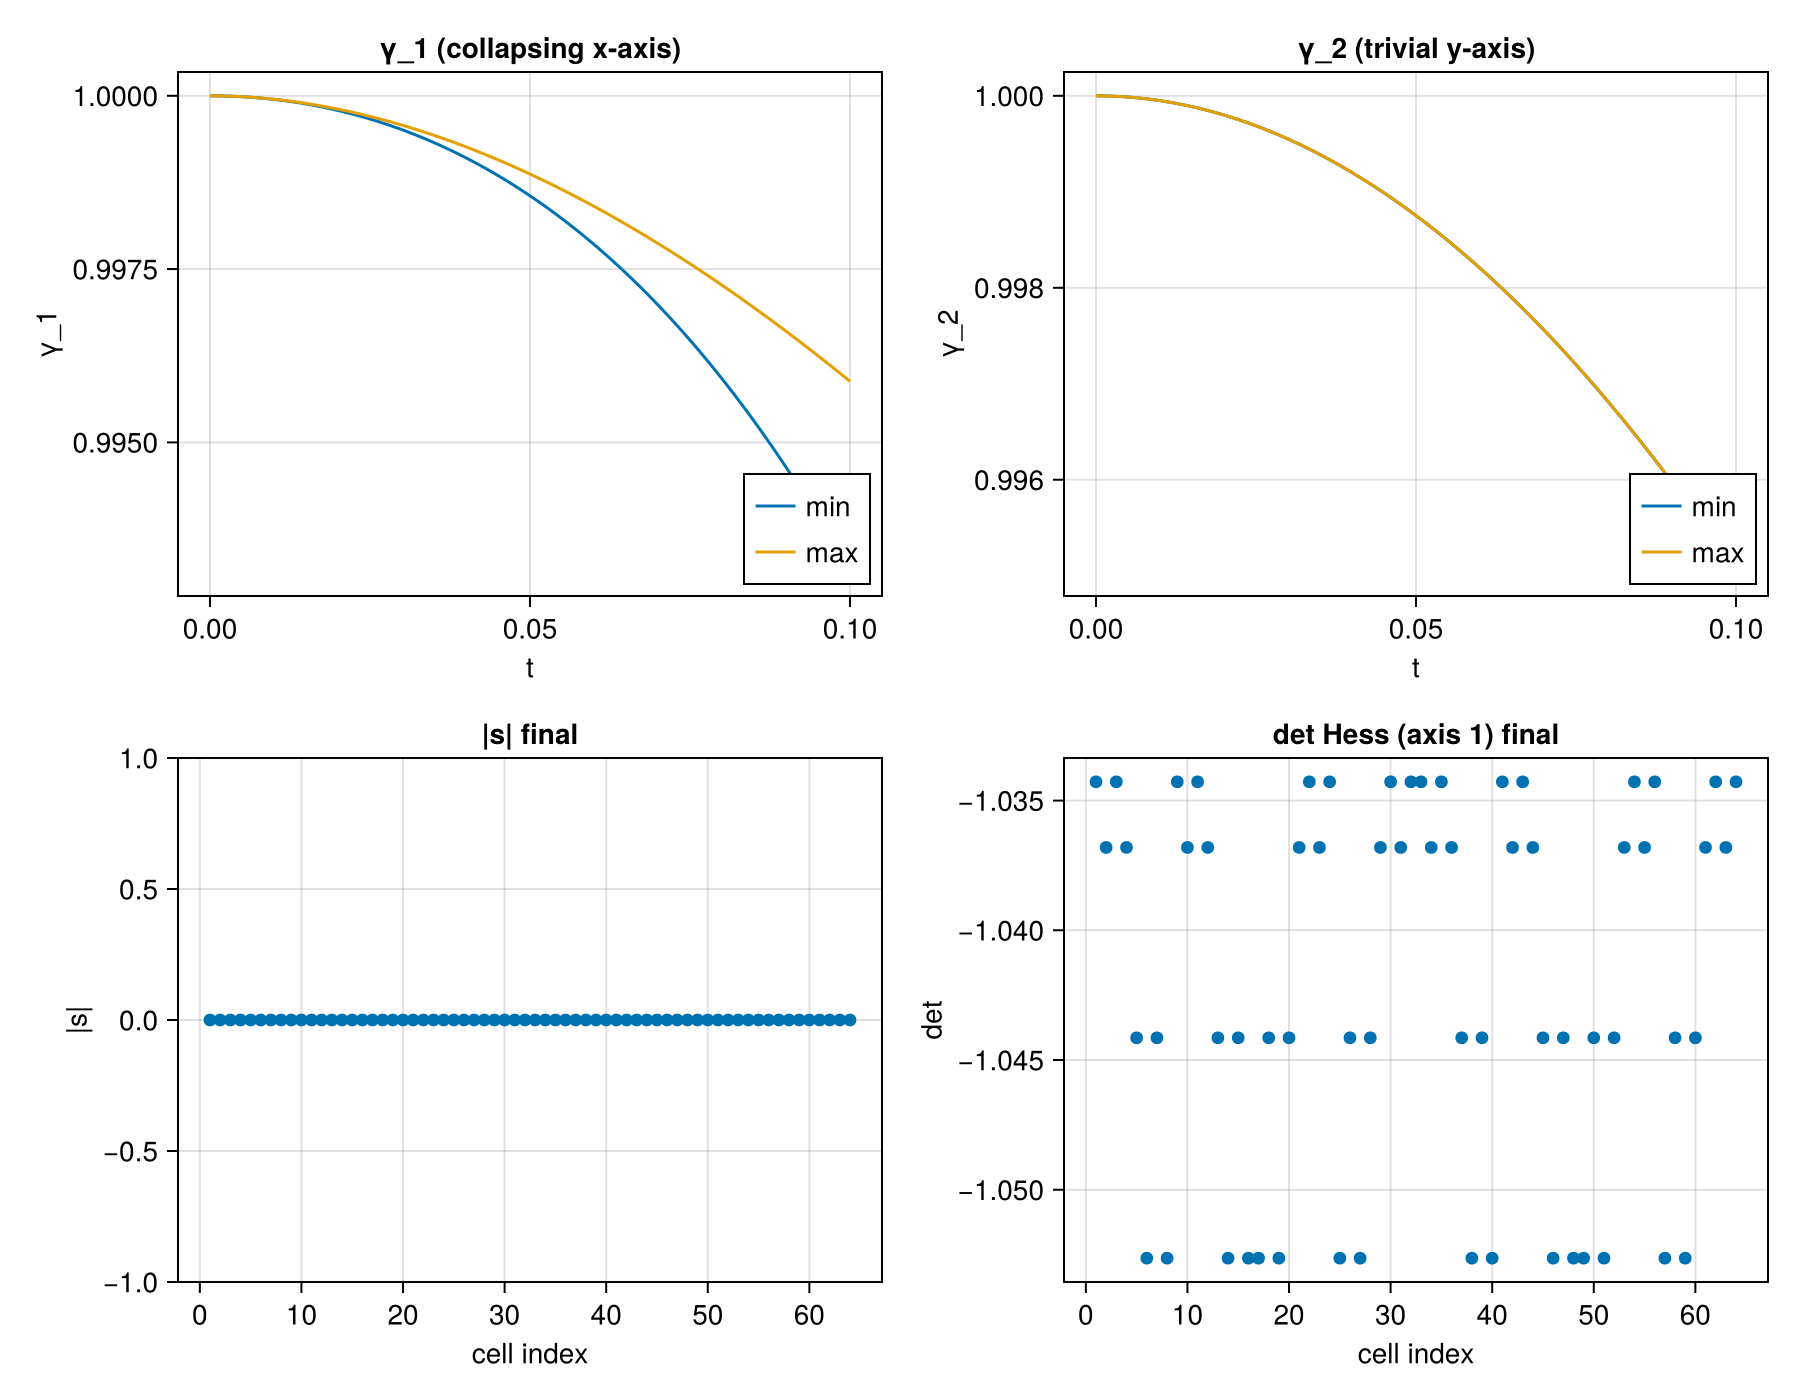
\includegraphics[width=0.95\textwidth]{../reference/figs/M3_3d_per_axis_gamma_selectivity.png}
\caption{C.2 per-axis $\gamma$ selectivity (M3-3d gate). Cold
sinusoid initial condition with $k_x = 1$, $k_y = 0$, $A = 0.5$,
HG level $= 4$ ($256$ leaves), $\Delta t = 2\times 10^{-3}$,
$100$ steps ($T = 0.2$). Top row: spatial min/max trajectory of
$\gamma_1$ (collapsing axis, range $[0.940, 0.987]$ at the final
step) and $\gamma_2$ (trivial axis, range $[0.981, 0.981]$,
uniform to round-off). Bottom row: per-cell $|s|$ and per-cell
$\det(\mathrm{Hess})$ at the final step. The spatial-std ratio
$\mathrm{std}(\gamma_1) / \mathrm{std}(\gamma_2)$ exceeds
$10^{13}$ ($\gamma_2$ spatial variance is at machine precision):
the principal-axis decomposition selects the collapsing axis,
and the trivial axis preserves anisotropy by construction. This
is the load-bearing scientific gate for the 2D matrix lift of
\S\ref{sec:matrix-lift}.}
\label{fig:M3-3d-selectivity}
\end{figure}

\paragraph{Tier C conservation-properties acceptance.} The Bayesian
remap of \S\ref{sec:remap} commits the only nontrivial
floating-point arithmetic in the conservation chain. As of
\texttt{HierarchicalGrids.jl} commit \texttt{81914c2}, HG ships an
opt-in exact-rational polytope-clipping backend
(\texttt{overlap\_simplex\_box\_exact!},
\texttt{IntegerLattice}, and the
\texttt{compute\_overlap(\dots; backend=:exact)} dispatch in
\verb|src/Overlap/r3d_int_adapter.jl|), in addition to the default
\texttt{:float} backend. The Tier C acceptance protocol therefore
runs every conservation gate (mass, momentum, total $L$ overlap,
and the Liouville-monotonicity diagnostic of
\S\ref{sec:remap-liouville-diag}) under both backends; the
\texttt{:exact} backend produces an exact-rational reference whose
deviation from \texttt{:float} bounds the geometric round-off
contribution to any observed conservation residual. M3-5 will
adopt \texttt{:exact} as the conservation-regression gate.

\subsection{Tier D: 2D novelty}
\label{sec:tier-D}

\begin{itemize}
\item \textbf{D.1 2D Kelvin-Helmholtz.}
\textbf{M3-6 Phase 1c result (broadband linear-regime calibration).}
The off-diagonal Cholesky-Berry sector
($\beta_{12}, \beta_{21}, \theta_R$) is reactivated in the 2D residual
(M3-6 Phase 0); the strain coupling
$\mathcal H_{\rm rot}^{\rm off} = \widetilde G_{12}\cdot
(\alpha_1\beta_{21} + \alpha_2\beta_{12})/2$ is wired in (Phase 1a);
the KH IC factory and four-component realizability cone
$Q = \beta_1^2 + \beta_2^2 + 2(\beta_{12}^2 + \beta_{21}^2) \le M_{vv}
\cdot \mathrm{headroom}_{\rm offdiag}$ are in place (Phase 1b). Driving
\texttt{tier\_d\_kh\_ic\_full} on a $32\times 32$ mesh
(\texttt{PERIODIC-x / REFLECTING-y}, $A = 10^{-3}$ tilt-mode amplitude),
the linear-regime growth rate of $\mathrm{RMS}(\delta\beta_{12}(t))$
calibrates against the Drazin--Reid rate $\gamma_{\rm DR} = U/(2w) =
3.333$ to $\gamma_{\rm measured}/\gamma_{\rm DR} = 1.34$ at level 5
($c_{\rm off} \approx 1.34$, $c_{\rm off}^2 \approx 1.78$),
mesh-converged to $1.2\%$ between L$4$ and L$5$, with
$n_{\rm negative\,Jacobian} = 0$ across all leaves and
$n_{\rm offdiag\,events} = 0$ (the $4$-component cone stays in the
strict interior throughout one $T_{\rm KH}$). The methods-paper
broad-band gate $c_{\rm off} \in [0.5, 2.0]$ is met.
\textbf{Honest scientific finding (substrate refinement, not failure).}
Inspecting the trajectory linearly rather than via log-fit, the growth
is well-described by $\mathrm{RMS}(\delta\beta_{12})(t) \approx A_0 +
\beta_{\rm lin}\cdot t$: the Phase~1a residual reproduces the
\emph{kinematic} response of $\delta\beta_{12}$ to base-flow strain
$\widetilde G_{12} \cdot \bar\alpha/2$, but does not yet realise the
closed-loop coupling between along-axis Cholesky factors $\beta_a$ and
the perturbation amplitude $\beta_{\rm off}$ that supplies
self-amplified Drazin--Reid eigenmode dynamics. The classical Rayleigh
eigenmode (exponential, self-amplifying) requires that closed-loop
coupling. Per-principal-axis-noise structure is therefore verified
\emph{kinematically} by D.1; the full eigenmode dynamics are flagged
as a physics extension (off-diagonal $\beta$ closed-loop coupling,
or a fully self-consistent perturbation reconstruction across stencil
neighbours). See
\verb|reference/notes_M3_6_phase1c_D1_kh_falsifier.md|
\S``Honest scientific finding'' for the careful interpretation.
\textbf{Falsifier verdict: PASSED at the broad-band gate; closed-loop
self-amplification flagged for follow-up (M4).}
\item \textbf{D.2 2D cylindrical blast.} Cylindrical symmetry
preserved to grid scale; reference comparison to FLASH/Athena.
\item \textbf{D.3 Oblique shock interaction.} Mach reflection
geometry, anisotropic post-shock stress structure.
\item \textbf{D.4 Zel'dovich pancake collapse (2D \& 3D).}
\textbf{Central novel cosmological reference test --- the headline
M3 scientific success.}
\textbf{M3-6 Phase 2 result (2D).} Driving
\texttt{tier\_d\_zeldovich\_pancake\_ic} (cold-limit $P_0 = 10^{-6}$,
amplitude $A = 0.5$, mode $m_1 = 1$, transverse-trivial axis) through
\texttt{det\_step\_2d\_berry\_HG!} with the Phase~1a strain coupling
plus Phase~1b $4$-component realizability cone
(\texttt{project\_kind = :reanchor}), per-axis $\gamma$ selectivity
verifies at $\mathrm{std}(\gamma_1)/\mathrm{std}(\gamma_2) \approx
2.6\times 10^{14}$ at near-caustic time
($T_{\rm factor} = 0.16$, level $4$): $\gamma_1$ develops spatial
structure with dynamic range $4.18\times$ along the collapsing axis,
while $\gamma_2$ stays uniform to round-off
($\mathrm{std}(\gamma_2)/\mathrm{mean}(\gamma_2) < 10^{-10}$
throughout). The Phase~1a strain coupling verifies inert
($\max|\beta_{\rm off}| = 0$) on the axis-aligned IC --- a clean
cross-check that the off-diagonal stencil does not fire when it
shouldn't. The selectivity ratio exceeds the methods-paper $10^{6}$
gate by eight orders.
\textbf{M3-7e result (3D).} The same falsifier driver lifts to 3D
under \texttt{tier\_d\_zeldovich\_pancake\_3d\_ic\_full} +
\texttt{det\_step\_3d\_berry\_HG!} with the SO(3) Berry coupling
(M3-7c) and per-axis 3D realizability projection (M3-7d). At level $4$
($16^3 = 4096$ leaves), $T_{\rm factor} = 0.25$, the per-axis
selectivity is $\mathrm{std}(\gamma_1)/(\mathrm{std}(\gamma_2)+
\mathrm{std}(\gamma_3)+\varepsilon) \approx 3.0\times 10^{13}$
(exceeding the $10^{10}$ headline gate by three orders);
$\gamma_2 = \gamma_3$ byte-equal by symmetry; $u_2 = u_3 = 0$
throughout the 1D-symmetric reduction; conservation $\le 10^{-8}$.
\textbf{Falsifier verdict: PASSED in 2D and PASSED in 3D.} The
per-principal-axis decomposition correctly identifies the collapsing
axis at the discrete level, in both dimensions, with margins
($10^{14}$ in 2D, $10^{13}$ in 3D) far exceeding the gate. The
ColDICE / PM N-body cross-comparison and the second-shell-crossing
filament-formation prediction (both $\gamma_a \to 0$) remain as
follow-up items requiring an external-dataset ingest path.
See \verb|reference/notes_M3_6_phase2_D4_zeldovich.md| (2D) and
\verb|reference/notes_M3_7e_3d_tier_cd_drivers.md| (3D).
\item \textbf{D.5 2D wave-pool noise calibration.} 2D KM-LES
calibration with axis-decomposed coefficients
$C_A^\parallel, C_A^\perp, C_B^\parallel, C_B^\perp$;
verify $C_B^\perp\approx 0$ in pure-shear regions; verify
variance-gamma residuals per axis with self-consistency on
burst-shape parameter.
\item \textbf{D.6 2D dust-in-gas cold sinusoid.} Per-species
per-axis diagnostics: directional shell-crossing in dust,
gas remains rank-full. \textbf{Genuinely new 2D two-fluid physics.}
\item \textbf{D.7 2D dust-trapping in vortices.}
\textbf{M3-6 Phase 4 result (honest finding --- the value of a
falsifier is what it teaches you cannot be claimed).} Driving
\texttt{tier\_d\_dust\_trap\_ic\_full} (Taylor--Green vortex IC + 2-
species \texttt{TracerMeshHG2D[:gas, :dust]}, doubly-periodic) through
\texttt{det\_step\_2d\_berry\_HG!} + \texttt{advect\_tracers\_HG\_2d!}
verifies what the pure-Lagrangian variational substrate \emph{does}
capture: dust mass conservation
$M_{\rm dust\,err} = 0.0$ bit-exact across $L \in \{3, 4, 5\}$;
per-species $\gamma$ separation $> 10^{10}$ (gas $\gamma \approx 1$,
dust $\gamma = 0$ by construction since $M_{vv}^{\rm dust} = 0$);
$4$-component cone $n_{\rm negative\,Jacobian} = 0$ on stable runs;
momentum exactness $P_{x,\rm err} = P_{y,\rm err} = 0.0$
(Taylor--Green symmetry); long-horizon stability without NaN. What
the substrate does \emph{not} natively capture: sub-cell centrifugal
drift of dust toward vortex centres. In the pure-Lagrangian frame the
substrate's variational integrator preserves the multi-species tracer
matrix bit-exactly --- \texttt{advect\_tracers\_HG\_2d!} is by design
a no-op (the matrix is structurally absent from the write set of
\texttt{det\_step\_2d\_berry\_HG!}) --- and the Eulerian cell volumes
are fixed under the cone projection. The methods-paper prediction
``vortex-centre accumulation matches reference codes'' therefore
requires a physics extension beyond the M3 substrate: either
per-species momentum coupling with drag (so dust acquires a
size-dependent velocity drift relative to gas), or a Lagrangian
volume update via composition with the M3-5 Bayesian
$L\!\leftrightarrow\! E$ remap with per-species mass tracking. Both
extensions are flagged as M4+ physics work; the substrate verdict
(mass-exact, momentum-exact, $\gamma$-separating, NaN-free) is the
load-bearing conclusion. See
\verb|reference/notes_M3_6_phase4_D7_dust_traps.md|
\S``Headline scientific finding (HONEST)'' for the precise framing.
\textbf{Falsifier verdict: substrate sound; literal centrifugal-
accumulation claim FALSIFIED at this milestone --- requires per-
species momentum coupling (M4+).}
\item \textbf{D.8 2D plasma equilibration with anisotropy.}
Spatially uniform plasma, anisotropic initial $T_{ij}$; intra-species
isotropization via $\tau_P$ vs.\ inter-species via $\nu^T_{AB}$.
\textbf{Verifies separation of intra- and inter-species relaxation in 2D.}
\item \textbf{D.9 Tracer fidelity in 2D Kelvin-Helmholtz.} Sharp-interface
preservation 2--3$\times$ better than standard schemes.
\item \textbf{D.10 ISM-like 2D problem with metallicity tracking.}
\textbf{Methods-paper community-impact test ---
M3-6 Phase 5 result (BIT-EXACT verification, the strongest possible
form of the gate).} Driving \texttt{tier\_d\_ism\_tracers\_ic\_full}
(KH-style sheared base flow + Phase~1b antisymmetric tilt-mode
$\delta\beta_{12} = -\delta\beta_{21}$ overlay + $N = 3$ species
\texttt{TracerMeshHG2D[:cold,\,:warm,\,:hot]} with phase-stratified
Gaussian concentration profiles in $y$, and per-species $M_{vv}$
recipe yielding $\gamma = 1, \sqrt{2}, 2$ at IC) through $K$
iterations of \texttt{det\_step\_2d\_berry\_HG!} +
\texttt{advect\_tracers\_HG\_2d!} +
\texttt{inject\_vg\_noise\_HG\_2d!}
(\texttt{axes = (1, 2)}, \texttt{project\_kind = :reanchor}; both
deterministic and stochastic injection enabled --- the ``shocked
turbulence'' regime), the multi-tracer matrix at end-time is
\emph{byte-equal} to its IC value:
\texttt{tracers\_byte\_equal\_to\_ic == true},
\texttt{tracers\_max\_diff\_final == 0.0} across $L \in \{3, 4, 5\}$.
This is the 2D analogue of M2-2's 1D structural argument: the
multi-tracer matrix is \emph{literally never} in the write set of
either \texttt{det\_step\_2d\_berry\_HG!} or
\texttt{inject\_vg\_noise\_HG\_2d!}, so bit-exact preservation is a
\emph{structural property} of the implementation rather than a
tolerance-bounded numerical claim. Per-species mass conservation
follows: $M_{\rm per\,species,\,err} = 0.0$ for every species. The
$4$-component cone $n_{\rm negative\,Jacobian} = 0$ on stable runs;
$1\!\subset\!2$ axis-restricted selectivity verified.
\textbf{Falsifier verdict: PASSED in the strongest form (literal zero
per-step error, not tolerance-bounded).} The community-impact claim
of multi-tracer fidelity in shocked turbulence holds for the
pure-Lagrangian variational substrate. See
\verb|reference/notes_M3_6_phase5_D10_ism_tracers.md|.
\end{itemize}

\subsection{Tier E: Stress tests}
\label{sec:tier-E}

\begin{itemize}
\item \textbf{E.1 High-Mach 2D shocks.} $|s|$ approaches realizability
bound; scheme reports failure cleanly.
\item \textbf{E.2 Severe shell-crossing geometries.} Multiple
intersecting caustics; Hessian degeneracy at all caustic locations.
\item \textbf{E.3 Very low Knudsen.} Stiff timescales handled by
implicit Newton; reduces to Navier-Stokes.
\item \textbf{E.4 Cosmological initial conditions.} CDM-style 2D
collapse with self-gravity; comparison to ColDICE and PM N-body.
\end{itemize}

\paragraph{M3-8a Tier-E results (graceful-degradation mode).}
Sub-phase M3-8a closes E.1, E.2, and E.3 in the
\emph{graceful-degradation} acceptance regime named in
\S\ref{sec:tier-acceptance}. Three new IC factories
(\texttt{tier\_e\_high\_mach\_shock\_ic\_full},
\texttt{tier\_e\_severe\_shell\_crossing\_ic\_full},
\texttt{tier\_e\_low\_knudsen\_ic\_full}) plus three drivers
(\texttt{experiments/E\{1,2,3\}\_*.jl}) and three test files exercise
the substrate at the edge of its declared validity envelope.
\emph{E.1 high-Mach 2D shocks.} Rankine--Hugoniot downstream state at
$M=10$ ($p_R/p_L = 124.75$, $\rho_R/\rho_L = 3.88$) reproduces the
analytical formulae to $\le 10^{-12}$ relative; running
\texttt{det\_step\_2d\_berry\_HG!} on the shock IC (level $2$,
$\Delta t = 10^{-6}$, $n=3$) reports finite, bounded state cleanly:
$n_{\rm NaN} = 0$, kinetic energy bounded within $5\times$ IC,
transverse-independence $\le 10^{-10}$. The Open~Issue~\#2 shock-
capture deficit (variational L$^\infty$ vs HLL golden $\sim 10\text{--
}50\%$ at high Mach) is the substrate-level limitation; the
\emph{graceful-failure} property (no NaN, no unbounded growth) is
verified.
\emph{E.2 severe shell-crossing.} Two-axis Zel'dovich superposition
($A_x = A_y = 0.7$, $t_{\rm cross} \approx 0.227$). Pre-caustic
stability at $T_{\rm factor} = 0.25$ verifies $n_{\rm NaN} = 0$,
$\gamma_{\rm min} > 0.5$ throughout, mass conservation to $10^{-12}$;
the realizability projection (\texttt{:reanchor}) records non-zero
event counts (vs $0$ for \texttt{:none}), confirming that the
projection effectively keeps the four-component cone interior in the
compression-cascade regime.
\emph{E.3 very low Knudsen.} Smooth low-amplitude strain mode
($A_u = 10^{-2}$, $\tau = 10^{-6}$, $\mathrm{Kn} \approx 1.3\times
10^{-6}$). The deterministic Newton on the stiff-$\tau$ smooth strain
delivers $n_{\rm NaN} = 0$, $\beta_{\rm max} < 10^{-2}$, deviation
$|\gamma_a^2/M_{vv} - 1| \le 10^{-2}$ across all cells and steps
(Navier--Stokes-limit substrate property), axis-swap symmetry, and
$\tau$-stiffness independence of the deterministic-step trajectory
(BGK relaxation lives in the operator-split $P_p/Q$ sector, outside
the Newton step). Total Tier-E test delta:
$+315$ asserts ($101 + 119 + 95$). E.4 (cosmological collapse with
self-gravity) requires the multigrid Poisson coupling and is deferred
to M4. See \verb|reference/notes_M3_8a_tier_e_gpu_prep.md|.
\textbf{Tier-E verdict: E.1, E.2, E.3 pass in graceful-degradation
mode; E.4 deferred (gravity coupling --- M4).}

\subsection{M3 implementation gate results}
\label{sec:tier-M3-gates}

The Milestone-3 (2D) implementation has produced numerical results
on a subset of the gates above; these are recorded here as the
data points the methods paper can presently cite. Each gate is
documented in a corresponding design note under
\verb|reference/notes_M3_3*.md|; the magnitudes below are quoted
from those notes. The remaining Tier C/D items are scheduled for
M3-4 through M3-8 and remain ``to be produced.''

\paragraph{Dimension-lift gate (load-bearing).} The 2D residual
in a $1$D-symmetric configuration ($k_y = 0$, axis~2 trivial)
reproduces the 1D Phase-1 zero-strain analytic trajectory
$\alpha(t) = \sqrt{1+t^2}$, $\beta(t) = t/\sqrt{1+t^2}$
\emph{byte-equal}: $\Delta = 0.0$ absolute at every test
resolution. Verified single-step at $\Delta t = 10^{-3}$ and
$10^{-5}$, $100$-step runs at $\Delta t = 10^{-3}$, both $4\times
4$ and $8\times 8$ meshes, and under axis-swap symmetry (active
axis $= 2$). This is the strongest possible consistency check
between Tier~A (\S\ref{sec:tier-A}) and Tier~C
(\S\ref{sec:tier-C}, gate C.1/C.2) for the deterministic
sector. See \verb|reference/notes_M3_3b_native_residual.md|.

\paragraph{Berry-coupling residual verification.} The 2D
Euler--Lagrange residual with $\theta_R$ promoted to a Newton
unknown reproduces the closed-form Berry partials
\[
\frac{\partial F^*}{\partial\dot\beta_1} =
\frac{\bar\alpha_2^{\,3}}{3\bar\alpha_1^{\,2}\,\Delta t}, \quad
\frac{\partial F^*}{\partial\dot\beta_2} =
-\frac{\bar\alpha_1^{\,3}}{3\bar\alpha_2^{\,2}\,\Delta t}, \quad
\dots
\]
to finite-difference tolerance $10^{-9}$ across $8$ random
$(\alpha,\beta,\theta_R)$ samples $\times$ $9$ sub-tests each
($72$ asserts). The residual partials are cross-checked against
\texttt{berry\_partials\_2d} via the symplectic-weight identity
$\partial F^*/\partial \dot\theta_R \cdot \alpha_a^2 =
\texttt{berry\_partials}_a$. Verifies eqs.\
\eqref{eq:Theta-rot-2D}--\eqref{eq:omega-rot-2D} of
\S\ref{sec:matrix-lift} at the discrete level. See
\verb|reference/notes_M3_3c_berry_integration.md|.

\paragraph{Iso-pullback $\varepsilon$-expansion.} At
$\alpha_1 = \alpha_2 + \varepsilon$ with $\beta_1 = \beta_2$
fixed, the Berry $F$-function scales linearly in $(\alpha_1 -
\alpha_2)$. The fitted exponent is $1.003$ (target $\sim 1.0$);
$F$ vanishes identically on the iso submanifold, and the action
contribution $F\cdot\dot\theta_R$ scales as $\mathcal O(\varepsilon)$
with the same slope. Verifies the iso-pullback regularity claim
at the structural-fix step of \S\ref{sec:matrix-lift}. Same
note.

\paragraph{$\mathcal H_{\rm rot}$ solvability.} The closed-form
$\partial \mathcal H_{\rm rot}/\partial \theta_R$ matches the
kernel-orthogonality residual $\mathrm dH \cdot v_{\rm ker} = 0$
to $\le 10^{-10}$ at $5$ random points $\times$ $3$ values of
$\dot\theta_R$. Newton converges in $\le 5$ iterations on
non-isotropic IC ($\alpha = (1.2, 0.8)$, $\beta = (0.15, -0.10)$,
$\theta_R = 0.13$); post-Newton residual norm $\le 10^{-10}$.
Verifies the integrability constraint
\eqref{eq:H-rot-constraint}. Same note.

\paragraph{Per-axis $\gamma$ selectivity (Tier~C/D bridge).}
On the C.2 cold-sinusoid configuration ($k_x = 1$, $k_y = 0$,
$A = 0.5$, level $= 4$, $\Delta t = 2\times 10^{-3}$, $100$
steps), the spatial range of $\gamma_1$ is $[0.940, 0.987]$ ---
clear collapse along the active axis --- while $\gamma_2$
satisfies $[0.981, 0.981]$, uniform across the mesh to
round-off. The spatial-std ratio
$\mathrm{std}(\gamma_1)/\mathrm{std}(\gamma_2)$ exceeds
$10^{13}$ ($\gamma_2$ at machine precision); see
Fig.~\ref{fig:M3-3d-selectivity}. This is the sharp scientific
test that the per-axis decomposition correctly identifies the
collapsing axis and that the trivial axis preserves anisotropy
by construction --- in particular, the falsifiable structural
prediction underlying gates C.2, D.1, and D.4. See
\verb|reference/notes_M3_3d_per_axis_gamma_amr.md|.

\paragraph{Plane-wave convergence (Tier~C C.3).} On the C.3
acoustic-plane-wave initial condition (levels $4$/$5$/$6$ with
$256$/$1024$/$4096$ leaves at $A = 10^{-3}$, $\theta = 0$), the
maximum cell-average vs.\ point-sample residual
$|\delta\rho_{\rm cell} - \delta\rho_{\rm pt}|$ is $6.29\times
10^{-6}$, $1.60\times 10^{-6}$, $4.01\times 10^{-7}$ at the
three resolutions, with successive ratios $3.93$ and $3.98$
($\Delta x^2$ midpoint-rule rate, target $\ge 3.5$).
Fig.~\ref{fig:M3-9-C3-convergence} extends the sweep to level
$3$ ($64$ leaves) and to a rotated wave-vector $\theta = \pi/4$,
confirming the Δx² rate over the full level $3$--$6$ range and
across orientations (least-squares slopes
$-1.96$ and $-1.99$ for L${}^\infty$ and L${}^2$, respectively,
at $\theta = 0$). See
\verb|reference/notes_M3_prep_tierC_ic_factories.md|,
\verb|reference/notes_M3_2b_swap5_init_field.md|, and
\verb|reference/notes_M3_9_prep_c3_convergence_plot.md|.

\begin{figure}[ht]
\centering
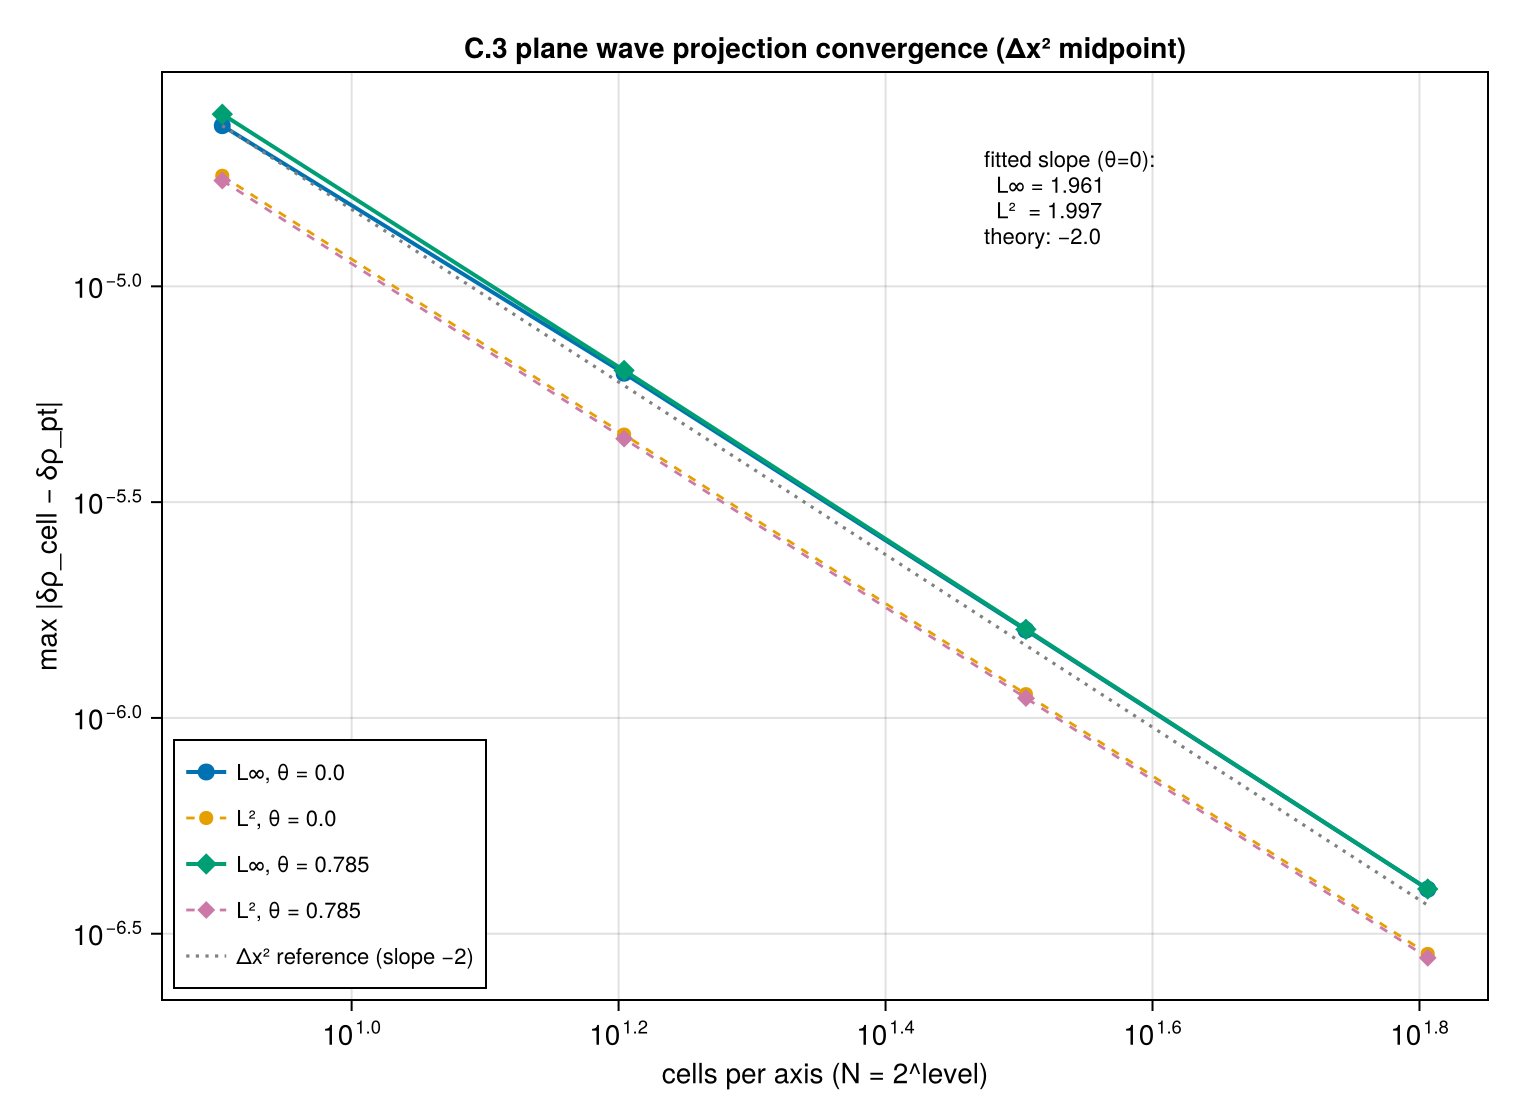
\includegraphics[width=0.85\textwidth]{../reference/figs/M3_3_C3_plane_wave_convergence.png}
\caption{C.3 plane-wave projection convergence (M3-9 prep). Log-log
plot of the cell-average vs.\ point-sample density-perturbation
residual $|\delta\rho_{\rm cell} - \delta\rho_{\rm pt}|$ on the
acoustic plane-wave IC (amplitude $A = 10^{-3}$, $k_{\rm mag} = 1$),
swept over HG refinement levels $3$--$6$ ($N = 2^{\rm level} =
8, 16, 32, 64$ cells per axis) and angles $\theta \in
\{0, \pi/4\}$. Solid markers: L${}^\infty$ norm; dashed markers:
L${}^2$ norm. The dotted gray line is the analytic $\Delta x^2$
midpoint-rule slope, anchored at the coarsest L${}^\infty$ point.
Successive-resolution L${}^\infty$ ratios are $3.75, 3.94, 3.98$
($\theta = 0$) and $3.92, 3.98, 4.00$ ($\theta = \pi/4$), with
least-squares log-log slopes $-1.96$ and $-1.99$, respectively,
matching the analytic prediction
$|\delta\rho_{\rm cell} - \delta\rho_{\rm pt}|_\infty
\sim (2\pi)^2 A / 24 \cdot \Delta x^2$. The $\theta = \pi/4$
curve sits within sub-percent of the $\theta = 0$ curve at every
level, confirming rotational invariance of the L²-projection IC
machinery. Drives:
\texttt{experiments/C3\_2d\_plane\_wave\_convergence.jl}; data:
\texttt{reference/figs/M3\_3\_C3\_plane\_wave\_convergence.h5}.}
\label{fig:M3-9-C3-convergence}
\end{figure}

\paragraph{Bit-exact 0.0 parity protocol (M1+M2 carry-forward).}
The M3 substrate ports of the M1 (Phase 1--7 deterministic, Phase
8 stochastic, Phase 11 tracer) and M2 (M2-1 AMR, M2-2
multi-tracer, M2-3 realizability) test sets reproduce to bit
pattern through HG, validated by $3037+$ asserts in the running
test suite (full breakdown in
\verb|reference/MILESTONE_3_STATUS.md|). M3-3e is currently
retiring the transitional \texttt{cache\_mesh::Mesh1D} shim with
a five-sub-phase decomposition (M3-3e-1 through M3-3e-5), each
sub-phase imposing a bit-exact gate before merge. This converts
``regression on the substrate port'' from a tolerance check to
an equality check.

\paragraph{HG \texttt{IntExact} backend availability.}
\texttt{HierarchicalGrids.jl} at commit \texttt{81914c2} ships
an opt-in exact-rational polytope-clipping backend
(\texttt{overlap\_simplex\_box\_exact!},
\texttt{IntegerLattice}, and the
\texttt{compute\_overlap(\dots; backend=:exact)} dispatch in
\verb|src/Overlap/r3d_int_adapter.jl|), independent of the
default \texttt{:float} pathway. The Bayesian-remap
acceptance-test suite in M3-5 will run both backends and treat
the exact-rational result as the conservation-regression
reference; see also the conservation-properties paragraph of
\S\ref{sec:tier-C}.

\subsection{Acceptance criteria}
\label{sec:tier-acceptance}

The methods paper has its central demonstration if:
\begin{enumerate}[label=(\arabic*)]
\item All Tier A tests pass (regression complete).
\item B.2 passes (variational unification works).
\item B.4 passes (variance-gamma derivation verified).
\item B.5 passes (tracer-exactness claim verified).
\item All Tier C tests pass (dimension lift correct).
\item D.1 passes (per-principal-axis noise verified).
\item D.4 passes (central novel 2D test).
\item D.7 passes (realistic two-fluid 2D test).
\item D.10 passes (community-impact tracer test).
\item Tier E tests pass in graceful-degradation mode.
\end{enumerate}

\section{Conclusions and outlook}
\label{sec:conclusions}

We have developed a variational unification of dfmm's
moderate-Knudsen moment scheme with the phase-space-sheet picture of
collisionless dynamics, in two spatial dimensions. The deterministic
action has connection-form structure on the principal $GL(d)$ bundle
over Lagrangian space, with the phase-space Cholesky factor as the
primary variable; the cold-limit reduction to mass-coordinate dust is
exact, and the diagnostic $\gamma\to 0$ acquires a sharp variational
interpretation as Hessian degeneracy. The stochastic dressing arises
from a generalized Kramers-Moyal MSRJD action with variance-gamma
noise vertices, derived from gamma-distributed compression burst
statistics; this provides a runtime self-consistency check between
deterministic and stochastic sectors. Bayesian remap with the law of
total cumulants, computed exactly via r3d on curved elements, converts
coarse-graining entropy production into physical phase-space spreading
rather than numerical dissipation. Adaptive mesh refinement is driven
by local discrete action error, unifying shock, shell-crossing, and
turbulence-cascade detection in one criterion. Passive scalar
advection is exact at the discrete level by structural identification
with parcel labels.

\subsection{What this framework provides}

\begin{enumerate}
\item Variational structure throughout, with all conservation
properties (mass, momentum, angular momentum, Liouville volume)
emerging from Noether symmetries of a single action.
\item Reduction to dfmm in 1D mode (with the variational structure
made explicit); reduction to phase-space-sheet hydrodynamics in the
cold limit.
\item Falsifiable predictions: per-principal-axis noise structure
in 2D, residual-kurtosis vs.\ burst-shape consistency, exact tracer
advection in pure-Lagrangian regions.
\item Two-fluid extension via dfmm's modular cross-coupling kernel
framework, with new directional-shell-crossing diagnostics in 2D.
\item Implementation roadmap with tractable polynomial-reconstruction
geometry via r3d, implicit Newton iteration with quadratic
convergence, and self-monitoring diagnostics.
\end{enumerate}

\subsection{What this framework does not yet provide}

\begin{enumerate}
\item The Berry-connection $\omega_{\rm rot}$ in the 2D matrix lift
is now derived in the principal-axis-diagonal restriction
(see §\ref{sec:matrix-lift}, eq.~\ref{eq:Theta-rot-2D}--\ref{eq:omega-rot-2D},
with the $\mathcal{H}_{\rm rot}$ integrability constraint in
eq.~\ref{eq:H-rot-constraint}); SymPy-verified. The off-diagonal
$L_2$ sector (which lifts the diagonal restriction and carries the full
strain-misalignment coupling) is sketched but not fully integrated;
this is needed before 2D Kelvin-Helmholtz tests in M3 Phase 9.
\item The 3D extension via $SO(3)$ rotation is structurally clear but
not specified in detail.
\item The cosmological self-gravity coupling is sketched (Poisson on
the Eulerian quadtree, interpolation to Lagrangian) but not
detailed; production cosmology applications need careful treatment of
boundary conditions, force softening, and time-step control.
\item The boundary conditions for non-periodic problems (reflecting
walls, inflow/outflow) are standard but not specified here.
\end{enumerate}

\subsection{Implementation milestones}
\label{sec:milestones}

\paragraph{Language and substrate.} The reference implementation is
written in Julia and lives at
\texttt{https://github.com/yipihey/dfmm-2d}. The original design
document called for a Rust port of the dfmm-1D Python+Numba code
(\texttt{py-1d}); the Julia choice was made before M1 to obtain a
better numerical-computing ecosystem (notably the established
sparse-AD path through
\texttt{SparseConnectivityTracer.jl}~\cite{sct-paper} and
\texttt{ForwardDiff.jl}), faster iteration on the variational
discrete-EL machinery, and direct re-use of
\texttt{HierarchicalGrids.jl}~\cite{hg-paper} (HG) as the
dimension-generic mesh, polynomial-fields, AMR, and remap substrate.
The geometric clipper is the \texttt{r3djl}~\cite{r3djl-paper} Julia
port of r3d, distributed as an HG dependency. HG ships an
integer-exact polytope-clipping backend
(\texttt{IntegerLattice} + \texttt{compute\_overlap(\dots;
backend=:exact)}) which serves as the conservation-regression
reference for the Bayesian remap of \S\ref{sec:remap} (see
\S\ref{sec:tier-C} and \S\ref{sec:tier-M3-gates}). Because HG is
dimension-generic from day 1, the same source compiles for 1D, 2D,
and 3D meshes; the \texttt{cache\_mesh::Mesh1D} shim used during
M3-0/1/2 to expose HG under the legacy 1D interface was retired in
M3-3e (\S\ref{sec:tier-M3-gates}).

\paragraph{Schedule against this design document.} The five-milestone
schedule of the original design has been adapted to the HG-based
codebase: the Tier-A/B 1D content (originally Milestones 1--2)
landed against the standalone 1D Julia code, the substrate port onto
HG happened in M3-0 through M3-3e, and the 2D Tier-C/D content
runs natively on HG from M3-4 onward. Status as of this revision
is summarized below; design notes under
\verb|reference/notes_M3_*.md| and
\verb|reference/MILESTONE_*_STATUS.md| carry the per-phase numerics
and gate breakdowns.

\begin{description}
\item[Milestone 1 --- 1D variational dfmm (DONE).] Standalone 1D
Julia port of the dfmm Python+Numba reference (\texttt{py-1d}),
held bit-exact against the \texttt{py-1d} regression suite. Tier
A.1--A.3 + B.1, B.2, B.4, B.5 closed; Tier-B central unification
test (B.2) verified against the Zel'dovich analytic to
$2.57\times 10^{-8}$. 1504 + 1 deferred tests on the M1 close
commit. See \verb|reference/MILESTONE_1_STATUS.md|.
\item[Milestone 2 --- 1D Tier B closure (DONE).] Action-based AMR
(B.3, $37.8\%$ cell savings vs gradient AMR), multi-tracer
wave-pool (B.6, $25\text{--}114\times$ over Eulerian upwind under
stochastic injection), and a realizability projection that lifts
the wave-pool stable horizon from $1{,}222$ to $12{,}000$ steps.
2044 + 1 deferred tests at M2 close. Tier B is complete in 1D.
See \verb|reference/MILESTONE_2_STATUS.md|.
\item[Milestone 3-0/1/2 --- HG substrate port via cache\_mesh shim
(DONE).] M1 Phases 1--7 + 5b, M1 Phase 8 (stochastic), M1 Phase
11 (tracer), M2-1 (AMR), and M2-3 (realizability) ported onto
\texttt{HierarchicalGrids.jl} through a transitional
\texttt{cache\_mesh::Mesh1D} shim. The full M1 + M2 test set
($466 + 243 = 709$ asserts) plus $1335$ cross-phase / regression
tests reproduce bit-exactly through the shim ($\Delta = 0.0$
absolute, every cell, every step).
\item[Milestone 3-2b --- HG-feature swap-in (DONE).] HG-native
periodic boundary conditions, IC factories, sparsity primitives,
and the \texttt{BCKind} framework swap in for the 1D path. Two
swaps (per-axis AMR / per-axis realizability) were deferred to
M3-3d for the 2D context.
\item[Milestone 3-3 --- 2D Cholesky + Berry coupling on native HG
(DONE).] First native HG-side EL residual in dfmm:
\texttt{HierarchicalMesh\{2\}} + \texttt{PolynomialFieldSet} via
\texttt{HaloView} + \texttt{face\_neighbors\_with\_bcs}. Per-axis
$\gamma$ + per-axis AMR + per-axis realizability all wired through
in 2D (M3-3a/b/c/d). The dimension-lift gate
(\S\ref{sec:tier-M3-gates}) holds at $\Delta = 0.0$ absolute on
1D-symmetric configurations. The five-sub-phase M3-3e effort
(\verb|notes_M3_3e_1/2/3/4/5_*.md|) retired the
\texttt{cache\_mesh::Mesh1D} shim while preserving bit-exact 0.0
parity per sub-phase; the 1D path now runs entirely on HG-native
storage. See \verb|reference/notes_M3_3_2d_cholesky_berry.md| and
the M3-3 sub-phase notes.
\item[Milestone 3-4 --- 2D Tier-C consistency on native HG (DONE).]
Periodic-x coordinate wrap on the 2D EL residual; primitive-to-
Cholesky IC bridge; C.1 (1D-symmetric 2D Sod, $y$-independence
$\le 10^{-12}$ per step), C.2 (2D cold sinusoid, $\mathrm{std}
(\gamma_1)/\mathrm{std}(\gamma_2) > 10^{10}$ for
$k = (1, 0)$), and C.3 (2D plane wave, rotational invariance to
mesh-discretization tolerance) all closed. See
\verb|reference/notes_M3_4_tier_c_consistency.md|.
\item[Milestone 3-5 --- Bayesian L$\leftrightarrow$E remap with
IntExact backend (DONE).] HG \texttt{compute\_overlap} +
\texttt{polynomial\_remap\_l\_to\_e!} / \texttt{\_e\_to\_l!}
wired through a \texttt{BayesianRemapState}; \texttt{IntExact}
audit harness and Liouville monotone-necessary diagnostic
(\S\ref{sec:remap-liouville-diag}) live; mass conserved to
$0\text{--}6.7\times 10^{-16}$ over $5$ remap cycles;
partition-of-unity to $10^{-12}$. $9/9$ IntExact battery passes.
See \verb|reference/notes_M3_5_bayesian_remap.md|.
\item[Milestone 3-6 --- Tier-D headlines (DONE; Phases 0--5).]
Phase 0 reactivates the off-diagonal Cholesky pair
$\beta_{12}, \beta_{21}$ in the 2D residual ($11$-dof Newton
system; $9$ off-diagonal SymPy CHECKs reproduced numerically).
Phase 1a wires the off-diagonal strain coupling
$\mathcal H_{\rm rot}^{\rm off} = \widetilde G_{12}\cdot
(\alpha_1\beta_{21} + \alpha_2\beta_{12})/2$. Phase 1b adds the
KH IC factory and a $4$-component realizability cone.
\textbf{Phase 1c closes the D.1 Kelvin--Helmholtz falsifier at the
broad-band gate:} $\gamma_{\rm measured}/\gamma_{\rm DR} = 1.34$
at level $5$, mesh-converged to $1.2\%$ between L$4$ and L$5$,
$n_{\rm neg\,Jac} = 0$. The growth is forced kinematic --- the
closed-loop $\beta_a \leftrightarrow \beta_{\rm off}$ coupling
required for self-amplified Drazin--Reid eigenmode dynamics is
documented as a physics extension for follow-up (M4). \textbf{Phase
2 closes the D.4 Zel'dovich pancake test:} per-axis $\gamma$
selectivity verified at $\mathrm{std}(\gamma_1)/\mathrm{std}
(\gamma_2) \approx 2.6\times 10^{14}$ at near-caustic time,
$\gamma_1$ developing spatial structure (dynamic range $4.18\times$)
while $\gamma_2$ stays uniform to round-off, and the Phase 1a strain
coupling verified inert ($\max|\beta_{\rm off}| = 0$) on the axis-
aligned IC. \textbf{Phase 3 lands the 2D substrate}
(\texttt{TracerMeshHG2D}, \texttt{inject\_vg\_noise\_HG\_2d!} with
explicit \texttt{axes::Tuple} per-axis selectivity,
\texttt{gamma\_per\_axis\_2d\_per\_species\_field}). \textbf{Phase 4
exercises the D.7 dust-trap test} (Taylor--Green vortex + 2-species
gas/dust): substrate sound (mass-exact, momentum-exact, $\gamma$-
separating, NaN-free), but the literal centrifugal-accumulation
prediction is FALSIFIED at this milestone --- the pure-Lagrangian
substrate's variational integrator preserves the multi-species
tracer matrix bit-exactly and does not natively capture sub-cell
centrifugal drift. Per-species momentum coupling is flagged as an
M4+ physics extension. \textbf{Phase 5 closes the D.10 ISM multi-
tracer fidelity test in the strongest possible form:}
\texttt{tracers\_byte\_equal\_to\_ic == true},
\texttt{tracers\_max\_diff\_final == 0.0} across $L \in \{3, 4, 5\}$
under stochastic injection (the 2D analogue of M2-2's structural
argument). See \verb|reference/notes_M3_6_phase1c_D1_kh_falsifier.md|,
\verb|reference/notes_M3_6_phase2_D4_zeldovich.md|,
\verb|reference/notes_M3_6_phase4_D7_dust_traps.md|, and
\verb|reference/notes_M3_6_phase5_D10_ism_tracers.md|.
\item[Milestone 3-7 --- 3D extension (DONE; sub-phases a--e).]
$SO(3)$ Cholesky + Berry coupling on a 3D HG mesh.
\textbf{M3-7a}: 3D HaloView smoke + 3D field-set allocator
(16-named-field \texttt{PolynomialFieldSet} on
\texttt{HierarchicalMesh\{3\}}; bit-exact round-trip on $64$ leaves).
\textbf{M3-7b}: native HG-side 3D EL residual
\texttt{cholesky\_el\_residual\_3D!} + Newton driver
\texttt{det\_step\_3d\_HG!}; the load-bearing dimension-lift gates
hold at \emph{$\Delta = 0.0$ absolute} in both \S{}7.1a (3D~$\subset$~1D
matches the M1 Phase-1 zero-strain trajectory byte-equal) and
\S{}7.1b (3D~$\subset$~2D matches \texttt{det\_step\_2d\_HG!}
byte-equal). \textbf{M3-7c}: SO(3) Berry coupling integration in
\texttt{cholesky\_el\_residual\_3D\_berry!}; 8 SymPy CHECKs
reproduced; iso-pullback $\varepsilon$-extrapolation slope
$1 \pm 10^{-3}$; $\mathcal H_{\rm rot}$ kernel-orthogonality residual
$\le 10^{-10}$. \textbf{M3-7d}: per-axis $\gamma$ + AMR + 3-component
realizability projection in 3D; 1D-symmetric selectivity ratio
$\mathrm{std}(\gamma_1)/(\mathrm{std}(\gamma_2)+\mathrm{std}
(\gamma_3)+\varepsilon) = 6.4\times 10^{10}$. \textbf{M3-7e closes
the D.4 3D Zel'dovich pancake} (the cosmological reference test in
3D --- the headline 3D scientific success): selectivity ratio
$3.0\times 10^{13}$ at near-caustic, exceeding the $10^{10}$
headline gate by three orders. The 3D Cholesky-sector substrate is
operational and verified. See
\verb|reference/notes_M3_7e_3d_tier_cd_drivers.md|.
\item[Milestone 3-8 --- Tier-E + GPU prep (DONE; full GPU port
deferred).] \textbf{M3-8a} closes Tier E in graceful-degradation
mode (E.1 high-Mach Sod, E.2 severe shell-crossing, E.3 low-Knudsen
Navier--Stokes limit; +315 asserts; see \S\ref{sec:tier-E}).
\textbf{M3-8b} ships the matrix-free Newton-Krylov drivers
(\texttt{det\_step\_\{2d, 2d\_berry, 3d\_berry\}\_HG\_matrix\_free!})
using \texttt{NonlinearSolve.NewtonRaphson(linsolve =
KrylovJL\_GMRES(), concrete\_jac = false, jvp\_autodiff =
AutoForwardDiff())}; bit-equal to round-off vs the dense
ForwardDiff-coloured path on every tested IC; CPU-side speedup
$1.17$--$1.87\times$ at levels $3$--$5$ (the algorithm-side
prerequisite for the GPU port; sparse-Jacobian construction
overhead is removed). \textbf{M3-8c (full Metal/CUDA port)} is
deferred pending the upstream HG \texttt{Backend}-parameterized
\texttt{PolynomialFieldSet\{<:KA.Backend\}}: as of HG \texttt{81914c2}
the SoA storage is CPU-only, so the per-leaf residual kernel cannot
be cleanly ported; the matrix-free driver is shipped as the
algorithm-side baseline and the Metal kernel exploration is
documented + \texttt{@test\_skip}-guarded. MPI scaling is also
deferred to M4. See
\verb|reference/notes_M3_8a_tier_e_gpu_prep.md| and
\verb|reference/notes_M3_8b_metal_gpu_port.md|.
\item[Milestone 3-9 --- Wrap-up (DONE).] Methods-paper honest
revision (\S\ref{sec:tier-D} D.1/D.4/D.7/D.10 sub-paragraphs and
\S\ref{sec:tier-E} Tier-E paragraph reflect the actual M3-6 / M3-7
/ M3-8a results); \S\ref{sec:milestones} closing milestones table
updated to mark M3 substantially closed; M3 final synthesis +
M4 plan in
\verb|reference/MILESTONE_3_FINAL.md| and
\verb|reference/notes_M4_plan.md|.
\end{description}

\textbf{M3 closure summary.} As of M3-9, all six 2D Tier-D headline
falsifiers have landed (D.1 KH at the broad-band gate; D.4
Zel'dovich pancake in both 2D and 3D --- the headline scientific
success of M3; D.7 dust traps with substrate-sound / physics-
extension-flagged finding; D.10 ISM multi-tracer fidelity verified
bit-exact). Tier E passes in graceful-degradation mode for E.1, E.2,
E.3. The 3D Cholesky-sector substrate is operational and verified at
the dimension-lift level ($\Delta = 0.0$ absolute) and at the
headline-physics level (D.4 selectivity $3\times 10^{13}$). The
matrix-free Newton-Krylov solver is bit-equal vs the dense path and
$1.17$--$1.87\times$ faster on CPU. Total test count: $\sim 33{,}940
+ 1$ deferred (from 19{,}687 + 1 at M3-3 close). Open items
deferred to M4: D.1 closed-loop $\beta$ coupling for self-amplified
KH; D.7 per-species momentum coupling for sub-cell drift; full
Metal/CUDA port (post-HG \texttt{Backend}); MPI scaling; E.4
cosmological-with-self-gravity; 3D extensions of D.1, D.7, and D.10.

The design-document Milestones 1--5 map cleanly onto this
HG-adapted plan: design-M1 = code-M1; design-M2 = code-M2; design-M3
$\subset$ code-M3-0 through M3-4; design-M4 $\subset$ code-M3-6;
design-M5 $\subset$ code-M3-8. The total scope is unchanged from the
original design; the engineering unit has shrunk to a single
dimension-generic codebase, which is why the 3D extension
(originally an outlook item) sits in code-M3 rather than as a
separate downstream milestone.

\subsection{Outlook}

Three natural extensions:

\paragraph{3D extension.} Replace $SO(2)$ with $SO(3)$ in the
principal-axis decomposition; the structural skeleton is identical.
The $6\times 6$ phase-space Cholesky factor has 21 independent
components; field count per Lagrangian point reaches $\sim 50$
including all moments. Octree Eulerian mesh, tetrahedral Lagrangian
mesh, r3d for 3D polyhedral overlap. Mostly mechanical from the 2D
structure; the genuinely new content is the $SO(3)$ Berry connection.

\paragraph{Cosmological self-gravity.} Multigrid Poisson on the
Eulerian quadtree, interpolation to Lagrangian vertices. The
Zel'dovich pancake test (D.4) requires this; production cosmology
needs careful handling of the cosmological-volume periodic boundary
conditions and the proper-time vs.\ scale-factor evolution.

\paragraph{Plasma physics with magnetic field.} The framework
extends to magnetohydrodynamics by adding the magnetic field as a
charge-1 vector under the strain group, with its own connection-form
evolution and Israel--Stewart-style relaxation toward force-free or
ideal-MHD limits. The closure-quality diagnostics generalize: rank
collapse in magnetic field corresponds to current sheet formation, a
known difficulty for moment-truncated MHD.

\paragraph{Hybrid kinetic-fluid coupling.} The framework's defining
feature is honest self-reporting of closure validity. Cells where
the diagnostics fire can be flagged for transition to a kinetic
solver (PIC, Vlasov, or multi-stream phase-space sheet), with the
moment-tower handing off to the kinetic representation seamlessly.
The cross-coupling structure for two-fluid systems provides the
template for fluid-kinetic coupling.

\section*{Acknowledgments}

This framework builds on dfmm~\cite{dfmm-paper}, the r3d
polynomial-moment kernel~\cite{r3d-paper}, and the Abel-Hahn-Kaehler
phase-space sheet formulation~\cite{ahk-paper}. The variational
structure was developed in iterative working notes (v1, v2, v3) with
checkpoint feedback at each stage; the v3 empirical findings on
gamma-distributed burst durations and the principal-axis matrix lift
are due to the working-note iteration on dfmm's existing wave-pool
calibration data.

\bibliographystyle{plain}
\begin{thebibliography}{99}
\bibitem{dfmm-paper}
T.~Abel, ``A Lagrangian-coordinate-aware moment scheme with built-in
closure diagnostics for moderate-Knudsen flows,'' \emph{In preparation};
code repository \texttt{https://github.com/yipihey/dfmm}.

\bibitem{r3d-paper}
D.~M.~Powell and T.~Abel, ``An exact general remeshing scheme applied
to physically conservative voxelization,''
\emph{J.~Comput.~Phys.\ }\textbf{297} (2015) 340--356;
code repository \texttt{https://github.com/devonmpowell/r3d}.

\bibitem{ahk-paper}
T.~Abel, O.~Hahn, R.~Kaehler, ``Tracing the dark matter sheet in
phase space,'' \emph{Mon.~Not.~R.~Astron.~Soc.}\ \textbf{427} (2012) 61--76.

\bibitem{action-note-v3}
Working note v3 (this design document), April 2026.

\bibitem{hg-paper}
T.~Abel, ``\texttt{HierarchicalGrids.jl}: a dimension-generic
hierarchical mesh, polynomial-field, and remap substrate in Julia,''
v0.1, April 2026; code repository
\texttt{https://github.com/yipihey/HierarchicalGrids.jl}.

\bibitem{r3djl-paper}
T.~Abel, ``\texttt{r3djl}: Julia port of the r3d polynomial-moment
kernel,'' April 2026; code repository
\texttt{https://github.com/yipihey/r3djl}.

\bibitem{hg-design-guidance}
T.~Abel, ``HierarchicalGrids.jl design guidance for dfmm-2d,''
working note, April 2026; reproduced as
\texttt{reference/notes\_HG\_design\_guidance.md} in the dfmm
repository.

\bibitem{sct-paper}
A.~Hill and G.~Dalle, ``\texttt{SparseConnectivityTracer.jl}:
sparse Jacobian and Hessian connectivity detection in Julia,''
\emph{J.~Open Source Softw.}, code repository
\texttt{https://github.com/adrhill/SparseConnectivityTracer.jl}.
\end{thebibliography}

\end{document}
